\documentclass[sigconf,nonacm]{acmart}

%% Enable subfigures
\usepackage{subfigure}
%% Enable numbers in scientific format.
\usepackage{siunitx}
%% Enable enumerate start from.
\usepackage{enumitem}

%% Enable theorems
\newtheorem{theorem}{Theorem}[section]
\newtheorem{lemma}[theorem]{Lemma}

%% Enable algorithms
\usepackage{algorithm}
\usepackage[noend]{algpseudocode}
\let\ReturnInline\Return
\renewcommand{\Return}{\State\ReturnInline}
\algrenewcommand\algorithmicrequire{$\rhd$}
\algrenewcommand\algorithmicensure{$\square$}

%% Fonts used in the template cannot be substituted; margin 
%% adjustments are not allowed.
\AtBeginDocument{%
  \providecommand\BibTeX{{%
    \normalfont B\kern-0.5em{\scshape i\kern-0.25em b}\kern-0.8em\TeX}}}

%% Rights management information.
\setcopyright{acmcopyright}
\copyrightyear{2018}
\acmYear{2018}
\acmDOI{XXXXXXX.XXXXXXX}

%% These commands are for a PROCEEDINGS abstract or paper.
\acmConference[Conference acronym 'XX]{Make sure to enter the correct
  conference title from your rights confirmation emai}{June 03--05,
  2018}{Woodstock, NY}
%% Title of the proceedings is different from ``Proceedings of ...''?
% \acmBooktitle{Woodstock '18: ACM Symposium on Neural Gaze Detection,
%  June 03--05, 2018, Woodstock, NY} 
% \acmPrice{15.00}
% \acmISBN{978-1-4503-XXXX-X/18/06}

%% Submission ID.
% \acmSubmissionID{123-A56-BU3}

%% Use the "author year" style of citations and references?
% \citestyle{acmauthoryear}

%% Message
\newcommand{\kk}[1]{{{\color{red} #1}}}
\newcommand{\ds}[1]{{{\color{blue} #1}}}
\newcommand{\su}[1]{{{\color{green} #1}}}

%% Ignore block
\newcommand{\ignore}[1]{}

%% Macros
\newcommand{\Lou}{\textit{Louvain}}
\newcommand{\LPA}{\textit{LPA}}
\newcommand{\Hyb}{\textit{Hybrid Louvain-LPA}}
\newcommand{\DelOrg}{\textit{$\Delta$-screening}}
\newcommand{\Del}{P-DDS}
\newcommand{\StaLou}{\textit{Static Louvain}}
\newcommand{\NaiLou}{$\text{P-ND}_\text{L}$}
\newcommand{\DelLou}{$\text{P-DDS}_\text{L}$}
\newcommand{\FroLou}{$\text{P-DF}_\text{L}$}
\newcommand{\StaLPA}{\textit{Static LPA}}
\newcommand{\NaiLPA}{$\text{P-ND}_\text{LPA}$}
\newcommand{\DelLPA}{$\text{P-DDS}_\text{LPA}$}
\newcommand{\FroLPA}{$\text{P-DF}_\text{LPA}$}
\newcommand{\FroHyb}{$\text{P-DF}_\text{H}$}

%% Short names (PR)
\newcommand{\Wbar}{Algorithm $\text{XX}_{\text{WBPR}}$}
\newcommand{\Barf}{Algorithm $\text{XX}_{\text{BFPR}}$}
\newcommand{\Sta}{Algorithm $\text{Static}_{\text{XXPR}}$}
\newcommand{\Nai}{Algorithm $\text{ND}_{\text{XXPR}}$}
\newcommand{\Tra}{Algorithm $\text{DT}_{\text{XXPR}}$}
\newcommand{\Fro}{Algorithm $\text{DF}_{\text{XXPR}}$}
\newcommand{\StaWbar}{Algorithm $\text{Static}_{\text{WBPR}}$}
\newcommand{\StaBarf}{Algorithm $\text{Static}_{\text{BFPR}}$}
\newcommand{\NaiWbar}{Algorithm $\text{ND}_{\text{WBPR}}$}
\newcommand{\NaiBarf}{Algorithm $\text{ND}_{\text{BFPR}}$}
\newcommand{\TraWbar}{Algorithm $\text{DT}_{\text{WBPR}}$}
\newcommand{\TraBarf}{Algorithm $\text{DT}_{\text{BFPR}}$}
\newcommand{\FroWbar}{Algorithm $\text{DF}_{\text{WBPR}}$}
\newcommand{\FroBarf}{Algorithm $\text{DF}_{\text{BFPR}}$}




\begin{document}

%% Full title of the paper.
\title[DF-PageRank: A Fast Incrementally Expanding and Contracting Approach for Updating PageRank on Dynamic Graphs]{DF-PageRank: A Fast Incrementally Expanding and Contracting Approach for Updating PageRank on Dynamic Graphs}

%% Short title to be used in page headers (optional).
% \title[short title]{full title}
% \subtitle{Something other than the title}

%% Authors and their affiliations.
\author{Subhajit Sahu}
\email{subhajit.sahu@research.iiit.ac.in}
\affiliation{%
  \institution{IIIT Hyderabad}
  \streetaddress{Professor CR Rao Rd, Gachibowli}
  \city{Hyderabad}
  \state{Telangana}
  \country{India}
  \postcode{500032}
}

%% Concise author list in page headers.
%\renewcommand{\shortauthors}{Sahu, Kothapalli, and Banerjee, et al.}

%% Show page numbers.
\settopmatter{printfolios=true}

%% Short summary of the work to be presented in the article.
\begin{abstract}
PageRank is a popular centrality metric that assigns importance to the vertices of a graph based on its neighbors and their score. Efficient parallel algorithms for updating PageRank on dynamic graphs is crucial for various applications, especially as dataset sizes have reached substantial scales. This technical report presents our Dynamic Frontier approach. Given a batch update consisting of edge insertions and deletions, it progressively identifies affected vertices that are likely to change their ranks with minimal overhead. On a server equipped with a 64-core AMD EPYC-7742 processor, our Dynamic Frontier PageRank outperforms Static, Naive-dynamic, and Dynamic Traversal PageRank by $7.8\times$, $2.9\times$, and $3.9\times$ respectively - on uniformly random batch updates of size $10^{-7}|E|$ to $10^{-3}|E|$. In addition, our approach improves performance at an average rate of $1.8\times$ for every doubling of threads.
\end{abstract}




%% The code below is generated by the tool at http://dl.acm.org/ccs.cfm.
\begin{CCSXML}
<ccs2012>
<concept>
<concept_id>10003752.10003809.10010170</concept_id>
<concept_desc>Theory of computation~Parallel algorithms</concept_desc>
<concept_significance>500</concept_significance>
</concept>
<concept>
<concept_id>10003752.10003809.10003635</concept_id>
<concept_desc>Theory of computation~Graph algorithms analysis</concept_desc>
<concept_significance>500</concept_significance>
</concept>
</ccs2012>
\end{CCSXML}

% \ccsdesc[500]{Theory of computation~Parallel algorithms}
% \ccsdesc[500]{Theory of computation~Graph algorithms analysis}

%% Pick words that accurately describe the work being presented.
\keywords{Parallel PageRank algorithm, Improved Dynamic Frontier approach}

% \received{20 February 2007}
% \received[revised]{12 March 2009}
% \received[accepted]{5 June 2009}




%% Process the author and title information.
\maketitle

\section{Introduction}
\label{sec:introduction}
Centrality metrics quantify the importance of nodes within a network based on link structures. PageRank \cite{rank-page99}, originally devised to rank web pages in search results, is one the most popular centrality metrics. It is based on the principle that pages receiving a greater number of high-quality links are of higher quality and, consequently, should be assigned higher ranks. Given the importance of such a metric, PageRank finds applications beyond web page ranking, including urban planning \cite{urban-zhang18}, traffic flow prediction \cite{traffic-kim15}, protein target identification \cite{banky2013equal}, evaluating the importance of brain regions \cite{zuo2012network}, identifying species crucial to environ\textit{mental} health \cite{allesina2009googling}, characterizing the properties of a software system \cite{chepelianskii2010towards}, and quantifying the scientific impact of researchers \cite{rank-senanayake15}. The growing availability of extensive interconnected / graph-based data has fueled substantial interest in parallel algorithms for computing PageRank \cite{rank-garg16, rank-nvgraph, rank-giri20, rank-guoqiang20, rank-li21, rank-sadi18, rank-sarma13}.\ignore{--- it has been implemented on multicore CPUs \cite{rank-garg16}, GPUs \cite{rank-nvgraph}, FPGAs \cite{rank-guoqiang20}, SpMV ASICs \cite{rank-sadi18}, CPU-GPU hybrids \cite{rank-giri20}, CPU-FPGA hybrids \cite{rank-li21}, and distributed systems \cite{rank-sarma13}.}

However, the dynamic nature of most real-world graphs, characterized by frequent edge insertions and deletions, poses challenges for recomputing PageRank from scratch, especially when dealing with small, rapid changes \cite{agarwal2012real, barros2021survey}. To address this, existing strategies instead iterate from ranks of vertices obtained in a previous snapshot of the graph, thereby reducing the required number of iterations for convergence. To further minimize the runtime needed, it is necessary to recompute only the ranks of vertices that are likely to change. One prevalent approach involves identifying reachable vertices from the updated regions of the graph and limiting processing to these vertices \cite{rank-desikan05, kim2015incremental, rank-giri20, sahu2022dynamic}. However, marking all reachable vertices as affected, even for minor rank changes, is likely to result in unnecessary computation. Further, updates may occur randomly, within dense graph regions --- necessitating processing a substantial portion of the graph. While our earlier work \cite{sahu2024incrementally} had addressed these issues on large dynamic graphs with uniformly random updates, we had observed that our proposed approach did not perform as well on real-world dynamic graphs --- parameter adjustment was needed to achieve acceptable performance. There is thus a need for a new approach that performs well on real-world dynamic graphs, where the nature of updates is different from a uniformly random update. In addition, to further improve performance, it is possible to halt rank updates for a vertex if its rank appears to have converged. This technical report introduces such an approach.




\subsection{Our Contributions}

This report introduces our Dynamic Frontier approach\footnote{\url{https://github.com/puzzlef/pagerank-openmp-dynamic}}, which, when given a batch update involving edge insertions and deletions, incrementally identifies affected vertices likely to undergo rank changes with minimal overhead. On a server equipped with a 64-core AMD EPYC-7742 processor, our Dynamic Frontier PageRank surpasses Static, Naive-dynamic, and Dynamic Traversal PageRank by $7.8\times$, $2.9\times$, and $3.9\times$ respectively, for uniformly random batch updates of size $10^{-7}|E|$ to $10^{-3}|E|$, where $|E|$ is the number of edges in the original graph. Additionally, our approach exhibits a performance improvement of $1.8\times$ for each doubling of threads. Additionally, our approach exhibits a performance improvement of $1.8\times$ for each doubling of threads.




%% - Use --- for a dash.
%% - Use ``camera-ready'' for quotes.
%% - Use {\itshape very} or \textit{very} for italicized text.
%% - Use \verb|acmart| or {\verb|acmart|} for mono-spaced text.
%% - Use \url{https://capitalizemytitle.com/} for URLs.
%% - Use {\bfseries Do not modify this document.} for important boldface details.
%% - Use \ref{fig:name} for referencing.

%% For a block of pre-formatted text: 
% \begin{verbatim}
%   \renewcommand{\shortauthors}{McCartney, et al.}
% \end{verbatim}

%% For a list of items:
% \begin{itemize}
% \item the ``ACM Reference Format'' text on the first page.
% \item the ``rights management'' text on the first page.
% \item the conference information in the page header(s).
% \end{itemize}

%% For a table:
% \begin{table}
%   \caption{Frequency of Special Characters}
%   \label{tab:freq}
%   \begin{tabular}{ccl}
%     \toprule
%     Non-English or Math&Frequency&Comments\\
%     \midrule
%     \O & 1 in 1,000& For Swedish names\\
%     $\pi$ & 1 in 5& Common in math\\
%     \$ & 4 in 5 & Used in business\\
%     $\Psi^2_1$ & 1 in 40,000& Unexplained usage\\
%   \bottomrule
% \end{tabular}
% \end{table}

%% For a full-width table:
% \begin{table*}
%   \caption{Some Typical Commands}
%   \label{tab:commands}
%   \begin{tabular}{ccl}
%     \toprule
%     Command &A Number & Comments\\
%     \midrule
%     \texttt{{\char'134}author} & 100& Author \\
%     \texttt{{\char'134}table}& 300 & For tables\\
%     \texttt{{\char'134}table*}& 400& For wider tables\\
%     \bottomrule
%   \end{tabular}
% \end{table*}


%% For inline math:
% \begin{math}
%   \lim_{n\rightarrow \infty}x=0
% \end{math},

%% For a numbered equation:
% \begin{equation}
%   \lim_{n\rightarrow \infty}x=0
% \end{equation}

%% For an unnumbered equation:
% \begin{displaymath}
%   \sum_{i=0}^{\infty} x + 1
% \end{displaymath}

%% For a figure:
% \begin{figure}[h]
%   \centering
%   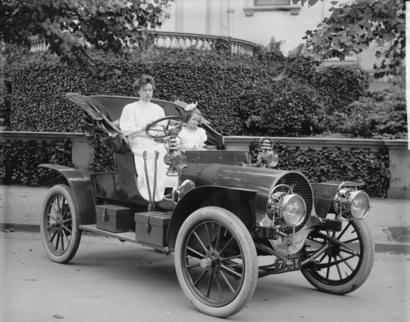
\includegraphics[width=\linewidth]{inc/sample-franklin}
%   \caption{1907 Franklin Model D roadster. Photograph by Harris \&
%     Ewing, Inc. [Public domain], via Wikimedia
%     Commons. (\url{https://goo.gl/VLCRBB}).}
%   \Description{A woman and a girl in white dresses sit in an open car.}
% \end{figure}

%% For a teaser figure.
% \begin{teaserfigure}
%   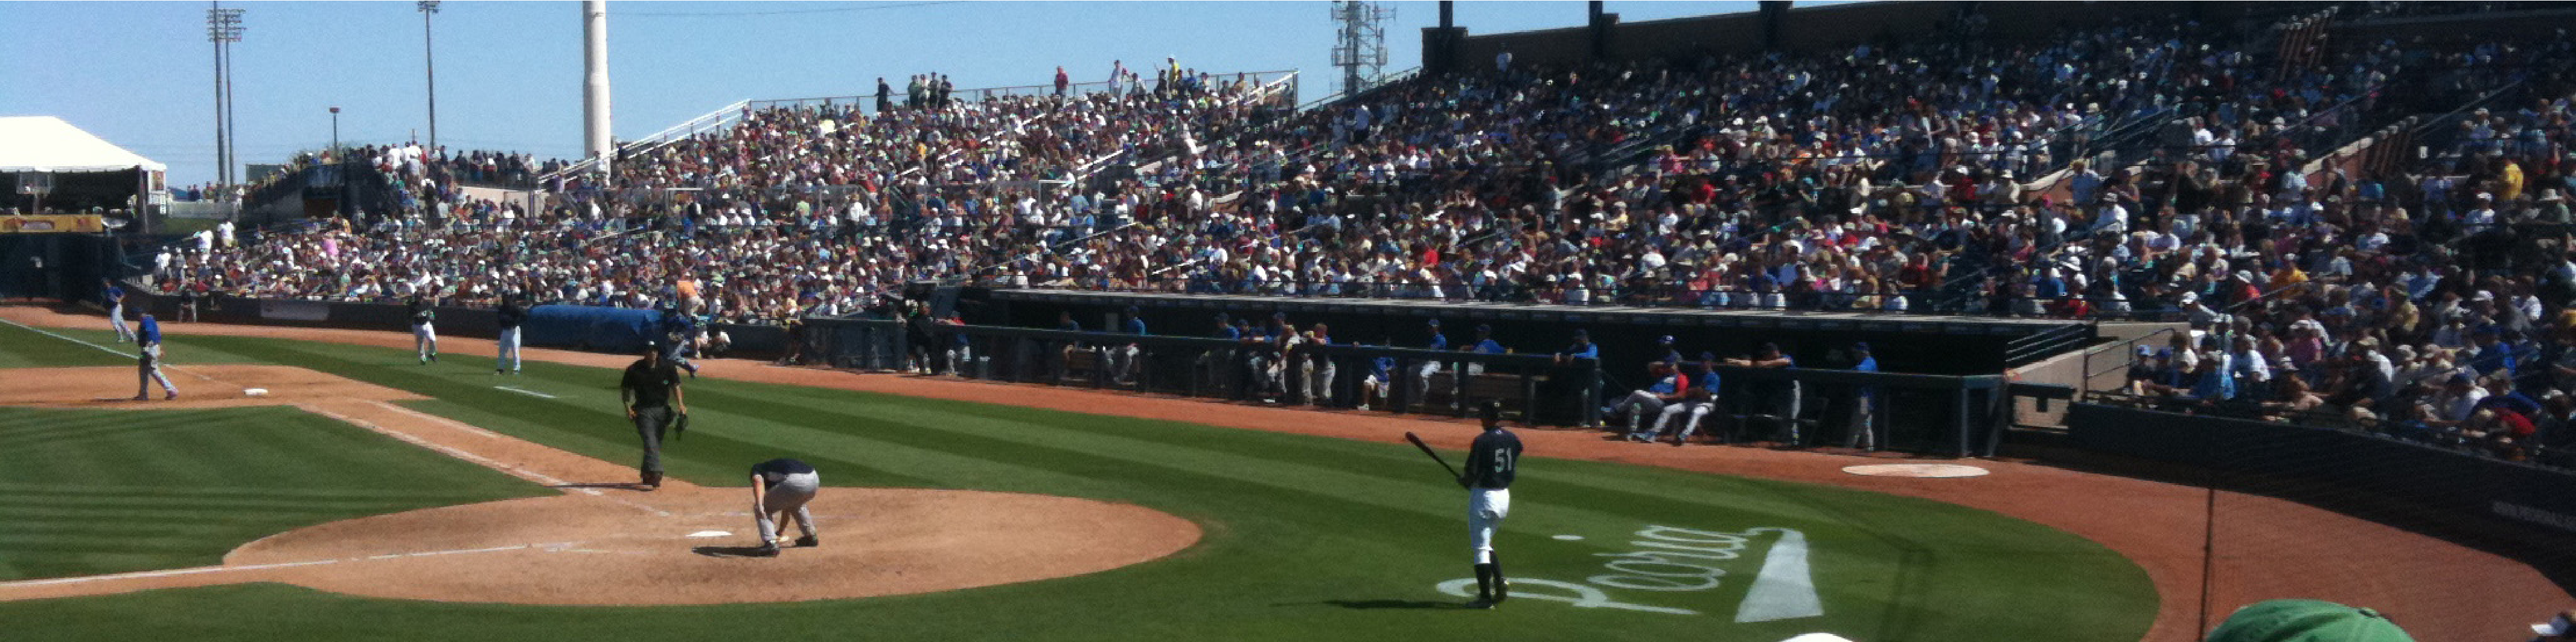
\includegraphics[width=\textwidth]{sampleteaser}
%   \caption{figure caption}
%   \Description{figure description}
% \end{teaserfigure}


\section{Related work}
\label{sec:related}
\ignore{Some of the early work on dynamic graph algorithms in the sequential setting include the seminal sparsification method of Eppstein et al. \cite{graph-eppstein97} and the bounded incremental computation idea of Ramalingam \cite{incr-ramalingam96}. The latter advocates measuring the work done as part of the update in proportion to the effect the update has on the computation.}

A number of approaches have been proposed for performing incremental computation (updating PageRank values in a dynamic / evolving graph) of approximate PageRank. Chien et al. \cite{rank-chien01} identify a tiny region of the graph near the updated vertices and model the remainder of the graph as a single vertex in a new, much smaller graph. PageRanks are computed for the small graph and then transferred to the original graph. Chen et al. \cite{chen2004local} propose a number of methods to estimate the PageRank score of a particular web page using only a small subgraph of the entire web, by expanding backwards from the target node following reverse hyperlinks. Bahmani et al. \cite{bahmani2010fast} analyze the efficiency of Monte Carlo methods for incremental computation of PageRank. Zhan et al. \cite{zhan2019fast} propose a Monte Carlo based algorithm for PageRank tracking on dynamic networks, by maintaining $R$ random walks starting from each node. Pashikanti et al. \cite{rank-pashikanti22} also follow a similar approach for updating PageRank scores on vertex and edge insertion/deletion.

A few approaches have been proposed for updating exact PageRank scores on dynamic graphs. Zhang \cite{rank-zhang17} presents a simple incremental Pagerank computation system for dynamic graphs on hybrid CPU and GPU platforms that incorporates the Update-Gather-Apply-Scatter (UGAS) computation model. A common approach used for Dynamic PageRank algorithm, given a small change to the input graph, is to find the affected region in the preprocessing step with Breadth-First Search (BFS) or Depth-First Search (DFS) traversal from the vertices connecting the edges that were inserted or deleted, and computing PageRanks only for that region \cite{rank-desikan05, kim2015incremental, rank-giri20, sahu2022dynamic}. This approach was originally proposed by Desikan et al. \cite{rank-desikan05}. Kim and Choi \cite{kim2015incremental} use this approach with an asynchronous implementation of PageRank. Giri et al. \cite{rank-giri20} use this approach with collaborative executions on muti-core CPUs and massively parallel GPUs. Sahu et al. \cite{sahu2022dynamic} use this approach on a Strongly Connected Component (SCC) based decomposition of the graph to limit the computation to SCCs that are reachable from updated vertices, on multi-core CPUs and GPUs (separately). Ohsaka et al. \cite{ohsaka2015efficient} propose an approach for locally updating PageRank using the Gauss-Southwell method, where the vertex with the greatest residual is updated first --- however, their algorithm is inherently sequential. 
%% Ohsaka et al. use L1-norm like many others for error.

% \ignore{PageRank algorithm is a \textbf{live algorithm} which means that an ongoing computation can be paused during graph update, and simply be resumed afterwards (instead of restarting it).} Dynamic PageRank algorithms aim to handle changes in the input graph efficiently.\ignore{A number of techniques have been proposed for online analysis of link evolution, i.e., updating of PageRank values in a dynamic/evolving graph.}

Further, Bahmani et al. \cite{rank-bahmani12} propose an algorithm to selectively crawl a small portion of the web to provide an estimate of true PageRank of the graph at that moment, while Berberich et al. \cite{rank-berberich07} present a method to compute normalized PageRank scores that are robust to non-local changes in the graph. Their approaches are orthogonal to our \textit{Dynamic Frontier} approach which focuses on the computation of the PageRank vector itself, not on the process of crawling the web or maintaining normalized scores.
%% Add other interesting variations?




%% COMPRE
%% ------
% Note that as originally conceived, the PageRank model does not factor a web browser's \textbf{back button} into a surfer's hyperlinking possibilities. Surfers in one class, if teleporting, may be much more likely to jump to pages about sports, while surfers in another class may be much more likely to jump to pages pertaining to news and current events. Such differing teleportation tendencies can be captured in two different \textbf{personalization vectors}. However, it makes the once query-independent, user independent PageRankings, user-dependent and more calculation-laden. Nevertheless, it seems this little personalization vector has had more significant side effects. This personalization vector, along with a \textbf{non-uniform/weighted} version of PageRank \cite{pr-dubey16} can help control spamming done by the so-called link farms \cite{pr-deeper01}.

% PageRank algorithms almost always take the following \textbf{parameters}: damping, tolerance, and maximum number of iterations allowed. Here, \textbf{tolerance} defines the error between the previous and the current iterations. Though this is usually $L_1$-norm, $L_2$ and $L_\infty$-norm are also used sometimes. Both damping and tolerance control the rate of convergence of the algorithm. The choice of tolerance function also affects the rate of convergence. However, adjusting \textbf{damping} can give completely different PageRank values. Since the ordering of vertices is important, and not the exact values, it can usually be a good idea to choose a larger tolerance value.

% Techniques to optimize the PageRank algorithm usually fall in two categories. One is to try \textbf{reducing the work per iteration}, and the other is to try \textbf{reducing the number of iterations}. Often, these goals are at odds against each other. The \textbf{adapting PageRank technique} "locks" vertices which have converged, and saves iteration time by skipping their computation \cite{pr-deeper01}. Identical nodes, which have the same in-links, can be removed to reduce duplicate computations and thus reduce iteration time. Road networks often have chains which can be short-circuited before PageRank computation to improve performance. Final ranks of chain nodes can be easily calculated. This reduces both the iteration time, and the number of iterations. If a graph has no dangling nodes, PageRank of each strongly connected component can be computed in topological order. This helps reduce the iteration time, number of iterations, and also enable concurrency in PageRank computation. The combination of all of the above methods is the \textbf{STIC-D algorithm} (see Figure \ref{fig:about-pagerank-sticd}) \cite{pr-sticd16}. A somewhat similar aggregation algorithm is \textbf{BlockRank} which computes the PageRank of hosts, local PageRank of pages within hosts independently, and aggregates them with weights for the final rank vector. The ranks of vertices for the entire graph can be found efficiently by computing the sub-PageRank of each connected component, and then using the sub-PageRanks together to form the global PageRank (Avrachenkov et. al. \cite{pr-avrachenkov04}). These methods exploit the inherent reducibility in the graph. The \textbf{Jacobi method} can also be used to compute the PageRank vector (Bianchini et. al. \cite{pr-bianchini05}) \cite{pr-deeper01}. \textbf{Monte Carlo} based PageRank methods consider several random walks on the input graph to get approximate PageRanks. Its optimizations for distributed PageRank computation (specially for undirected graphs) \cite{compute-frey13}, map-reduce algorithm for personalized PageRank \cite{pr-bahmani11}, and reordering strategy (to reduce space and compute complexity on GPU) for local PageRank \cite{pr-lai17} are present.

% The time per iteration can be reduced further by taking note of the fact that the traditional algorithm is \textbf{not computationally bound} and \textbf{generates fine granularity random accesses} (it exhibits irregular parallelism). This causes poor memory bandwidth and compute utilization, and the extent of this is quite dependent upon the graph structure \cite{compute-hunold15} \cite{pr-lakhotia18}. \textit{Four strategies for neighbour iteration} were attempted, to help reason about the \textit{expected impact of a graph's structure} on the performance of each strategy \cite{compute-hunold15}. CPUs/GPUs are generally designed optimized to \textbf{load memory} in blocks (cache-lines in CPUs, coalesced memory reads in GPUs), and not for fine-grained accesses. Being able to adjust this behaviour depending upon application (PageRank) can lead to performance improvements. Techniques like \textit{prefetching to SRAM, using a high-performance shuffle network} \cite{graph-wang15}, \textit{indirect memory prefetcher (of the form $A[B[i]]$), partial cache line accessing mechanisms} \cite{memory-yu15}, \textit{adjusting data layout} \cite{pr-lakhotia18} \textit{(for sequential DRAM access} \cite{pr-zhou15} \textit{), and branch avoidance mechanisms (with partitioning)} \cite{pr-lakhotia18} are used. Large graphs can be \textbf{partitioned }or decomposed into subgraphs to help reduce cross-partition data access that helps both in distributed, as well as shared memory systems (by reducing random accesses). Techniques like \textit{chunk partitioning} \cite{pr-rungsawang12}, \textit{cache/propagation blocking} \cite{pr-beamer17}, \textit{partition-centric processing with gather-apply-scatter model} \cite{pr-lakhotia18}, \textit{edge-centric scatter-gather with non-overlapping vertex-set} \cite{pr-zhou17}, \textit{exploiting node-score sparsity} \cite{pr-li21}, and even \textit{personalized PageRank based partitioning} \cite{pr-mazaheri19} have been used. Graph/subgraph \textbf{compression} can also help reduce memory bottlenecks \cite{pr-rungsawang12} \cite{pr-guoqiang20}, and enable processing of larger graphs in memory. A number of techniques can be used to compress adjacency lists, such as, \textit{delta encoding of edge/neighbour ids} \cite{graph-bharat98}, and \textit{referring sets of edges in edge lists} \cite{graph-adler01} \cite{graph-raghavan03} (hard to find reference vertices though) \cite{pr-deeper01}. Since the rank vector (possibly even including certain additional page-importance estimates) must reside entirely in main memory, a few compression techniques have been attempted. These include \textit{lossy encoding schemes based on scalar quantization} seeking to minimize the distortion of search-result rankings \cite{pr-haveliwala02} \cite{pr-deeper01}, and using \textit{custom half-precision floating-point formats} \cite{pr-molahosseini20}.

% As new software/hardware \textbf{platforms} appear on the horizon, researchers have been eager to test the performance of PageRank on the hardware. This is because each platform offers its own unique architecture and engineering choices, and also because PageRank often serves as a good benchmark for the capability of the platform to handle various other graph algorithms. Attempts have been made on distributed frameworks like \textit{Hadoop} \cite{pr-abdullah10}, and even \textit{RDBMS} \cite{compute-barolli21}. A number of implementations have been done on \textit{standard multicores} \cite{compute-barolli21}, \textit{Cell BE} \cite{compute-buehrer08} \cite{pr-zhou17}, \textit{AMD GPUs} \cite{pr-wu10}, \textit{NVIDIA/CUDA GPUs} \cite{pr-bisson16} \cite{pr-zhou17} \cite{graph-seo15}, \textit{GPU clusters} \cite{pr-rungsawang12}, \textit{FPGAs} \cite{pr-mughrabi21} \cite{graph-wang15} \cite{pr-guoqiang20}, \textit{CPU-FPGA hybrids} \cite{pr-hassan21} \cite{pr-usta21} \cite{pr-li21}, and even on SpMV \textit{ASICs} \cite{pr-sadi18}.

% PageRank algorithm is a \textbf{live algorithm} which means that an ongoing computation can be paused during graph update, and simply be resumed afterwards (instead of restarting it). The first \textbf{updating} paper by Chien et al. \cite{pr-chien01} identifies a tiny region of the graph near the changed vertices/edges and model the remainder of the graph as a single vertex in a new, much smaller graph. PageRanks are computed for the small graph and then transferred to the original graph \cite{pr-deeper01}. A common technique used for dynamic PageRank algorithm, given a small change to the input graph, is to find the affected region in the preprocessing step with breadth-first search (BFS) or depth-first search (DFS) traversal from the vertices connecting the edges that were inserted or deleted \cite{pr-desikan05} \cite{pr-giri20}.

  % 1 &
  % Prasanna Desikan, Nishith Pathak, Jaideep Srivastava, and Vipin Kumar. 2005. \textbf{Incremental page rank computation on evolving graphs}. In Special interest tracks and posters of the 14th international conference on World Wide Web (WWW '05). Association for Computing Machinery, New York, NY, USA, 1094–1095.\linebreak
  % DOI: https://doi.org/10.1145/1062745.1062885 &
  % 54 \\ \hline
  % \multicolumn{3}{|p{14cm}|}{This paper describes a simple method for computing dynamic pagerank, based on the fact that change of out-degree of a node does not affect its pagerank (first order markov property). The part of the graph which is updated (edge additions / edge deletions / weight changes) is used to find the affected partition of the graph using BFS. The unaffected partition is simply scaled, and pagerank computation is done only for the affected partition. \footnote{https://gist.github.com/wolfram77/f0a7534d49d5c07d4479ec3966c5d635}} \\ \hline

  % 2 &
  % Yen-Yu Chen, Qingqing Gan, and Torsten Suel. 2002. \textbf{I/O-efficient techniques for computing pagerank}. In Proceedings of the eleventh international conference on Information and knowledge management (CIKM '02). Association for Computing Machinery, New York, NY, USA, 549–557.\linebreak
  % DOI: https://doi.org/10.1145/584792.584882 &
  % 33 \\ \hline
  % \multicolumn{3}{|p{14cm}|}{This paper describes a technique to partition the link file of the whole file into blocks of a range of destination nodes, with partial source nodes, so that it is possible to run power iteration of pagerank of massive graphs which do not fit in memory. The graphs must be stored on disk, and partitions of the graphs are scanned in every iteration until the ranks converge. Unlike Haveliwala's technique, this is similar to pull based pagerank. Both methods have similarities with join techniques in database systems. Topic-sensitive pagerank is also discussed which finds pagerank of graphs related to a specific keywords beforehand, and merges them together based upon the query (might return better results than global pagerank). This requires small adjustments to the random jump probability factor $(1-d)$. \footnote{https://gist.github.com/wolfram77/925cede0214aa0f391f34fa8ce137290}} \\ \hline

  % 3 &
  % Paritosh Garg and Kishore Kothapalli. 2016. \textbf{STIC-D: algorithmic techniques for efficient parallel pagerank computation on real-world graphs}. In Proceedings of the 17th International Conference on Distributed Computing and Networking (ICDCN '16). Association for Computing Machinery, New York, NY, USA, Article 15, 1–10.\linebreak
  % DOI: https://doi.org/10.1145/2833312.2833322 &
  % 7 \\ \hline
  % \multicolumn{3}{|p{14cm}|}{In this paper, the authors exploit the reducibility of dead-end free graphs to compute PageRanks. They first split the vertices into strongly connected components (SCCs) and represent each SCC as a vertex in a block-graph. Each SCC is then processed as per its topological order in the block-graph. This enables them to reduce the operating memory requirement, thanks to the smaller size of SCCs that are processed in one go. As SCCs are processed in topological order, unnecessary iterations on vertices that are unlikely to converge are avoided. Processing vertices grouped into SCCs also improves performance due to inherent spatial locality within an SCC. In addition, this method allows SCCs residing on the same level in the block-graph to be processed independently of each other. This is demonstrated by the authors by processing each such SCC in parallel with OpenMP. They also present three algorithmic techniques for eliminating redundancies in PageRank computation, namely skipping repeated computation on in-identical vertices (minimize redundant computation), short circuiting chain vertices (help accelerate convergence), and skipping computation on vertices that appear to have converged (minimize redundant computation).The suitability of these techniques depend upon the nature of input graph. They study the techniques on four classes of real-world graphs: web graphs, social networks, citation and collaboration networks, and road networks. Their implementation achieves an average speedup of 32\% compared to a baseline implementation. \footnote{https://gist.github.com/wolfram77/bb09968cc0e592583c4b180243697d5a}} \\ \hline

  % 4 &
  % Stergios Stergiou. 2020. \textbf{Scaling PageRank to 100 Billion Pages}. Proceedings of The Web Conference 2020. Association for Computing Machinery, New York, NY, USA, 2761–2767.\linebreak
  % DOI: https://doi.org/10.1145/3366423.3380035 &
  % 1 \\ \hline
  % \multicolumn{3}{|p{14cm}|}{In this paper, the author exploits the fact the communication required between iterations is identical. He uses this to develop a new communication format that allows significant reduction in bandwidth requirement. He experiments on massive web graphs with up to 38 billion vertices and 3.1 trillion edges, requiring a per-iteration time of 34.4 seconds, which is more than an order of magnitude improvement over the state-of-the-art. \footnote{https://gist.github.com/wolfram77/10964cd26f11f7a7299e7b74a0be7e7e}} \\ \hline
%% ------

Coarse PageRank approaches: Arasu et al. \cite{rank-arasu02} proposed HostRank, where the web is aggregated at the level of host names. BlockRank \cite{kamvar2003exploiting} uses HostRank to initialize PageRank, while DirRank \cite{rank-eiron04} forms aggregation at the level of directories of websites.





%% We use an asynchronous approach:
% Real-Time PageRank on Dynamic Graphs (2023): In this paper, Sallinen et al. \cite{sallinen2023real} compute PageRank asynchronously for real-time, on demand PageRank computation with arbitrary granularity. They model PageRank as a flow problem, where mass is absorbed by the page, and the rest is distributed to neighbors. This is done by sending delta values of probability mass depending on edge deletion or insertions by adjustment upon earlier values. Sink/dangling vertices (dead ends) are handled as usual (teleport).

%% Interesting approach:
% PageRank Algorithm Based on Dynamic Damping Factor (2023): Existing methods often set the damping factor empirically, overlooking the relevance of web visitors’ topics. HaoLin et al. \cite{haolin2023pagerank} propose an adaptive dynamic damping factor based on the web browsing context, and demonstrate that it effectively mitigates the impact of noisy web pages on query results and improves the convergence speed.

%% Sliding window approach.
% Time-Aware Ranking in Dynamic Citation Networks (2011): In this paper, Ghosh et al. \cite{ghosh2011time} consider the temporal order of links and chains of links connecting to a node with some temporal decay factors, and show that it is more appropriate for predicting future citations and PageRank scores with regard to new citations.

%% Other interesting approach:
% A Dynamical System for PageRank with Time-Dependent Teleportation (2014): In this paper, Gleich and Rossi \cite{gleich2014dynamical} propose a time-dependent teleportation to the PageRank score. The magnitude of the deviation from a static PageRank vector is given by a PageRank problem with complex-valued teleportation parameters. They demonstrate the utility of dynamic teleportation on both the article graph of Wikipedia, where the external interest information is given by the number of hourly visitors to each page, and the Twitter social network, where external interest is the number of tweets per month. They show that using information from the dynamical system helps improve a prediction task and identify trends in the data.

%% Other interesting approach:
% Temporal PageRank (2016): In this paper, Rozenshtein and Gionis \cite{rozenshtein2016temporal} propose an extension of static PageRank to temporal PageRank so that only temporal walks are considered instead of all possible walks. In order to compute temporal PageRank we need to process the sequence of interactions and calculate the weighted number of temporal walks. Their algorithm counts explicitly the weighted number of temporal walks.

%% Similar to STIC-D:
% Divide and conquer approach for efficient pagerank computation (2006): In this paper, Desikan et al. \cite{desikan2006divide} propose a graph-partitioning technique for PageRank, on which computation can be performed independently.

%% Similar to STIC-D:
% A componentwise PageRank algorithm (2015): In this paper, Engstrom et al. \cite{engstrom2015componentwise} propose two PageRank algorithms, one similar to the Lumping algorithm proposed by Qing et al. which handles certain types of vertices faster, and last, another PageRank algorithm which can handle more types of vertices as well as strongly connected components more effectively. This is similar to the work of Garg et al.

%% Streaming PageRank:
% Estimating PageRank on graph streams (2011): In this paper, Sarma et al. \cite{rank-sarma11} study the streaming model for PageRank, which uses a small amount of memory (preferably sub-linear in the number of nodes n). They compute approximate PageRank values in Õ(nM−1/4) space and Õ(M3/4) passes. They also give another approach to approximate the PageRank values in just Õ(1) passes although this requires Õ(nM) space.

%% Applications of PageRank:
% PageRank Tracker: From Ranking to Tracking (2013): PageRank has been used by Gong et al. \cite{gong2013pagerank} in video object tracking to improve its robustness, i.e., to address difficulties with adaptation to environmental or target change. Determining the target is equivalent to finding the unlabeled sample that is the most associated with the existing labeled set.

%% Applications of PageRank:
% Abstracting PageRank To Dynamic Asset Valuation (2006): In this paper, Sawilla \cite{sawilla2006abstracting} uses (weighted) PageRank to quickly and dynamically calculate a relative value for all assets in an organization in any context in which dependencies may be specified. Their scheme works in general and will provide asset valuation in any context, be it confidentiality, integrity, availability, or even political capital.

%% For introduction, also a bit here:
% Adaptive Implementation to Update Page Rank on Dynamic Networks (2021): In this oral presentation, Srinivasan \cite{srinivasan2021adaptive} talk about the fact that There are a lot of attempts made to parallelize the page rank algorithm for static networks, however, there are only very few attempts made to compute page rank on dynamic networks. As the networks change with time, computing page rank or updating is an expensive operation, the previous attempts have only approximated the metric to avoid recomputation. In this paper, we introduce a framework where we try to update the page rank of the vertices which embraces change as the network changes. The proposed framework is implemented on a shared memory system and experiments on real-world and synthetic networks show good scalability. The framework proposed gets an input set of networks, initial page rank values for all the vertices, and a set of batches that has the changeset. As the batches are processed in parallel, affected vertices are identified and marked for an update, once the batch is processed the vertices affected or identified their page rank values are computed. The main contribution of this paper is the proposed framework avoids recomputation of all vertices, and only recomputes few vertices, and avoids approximation to provide accurate values.


\section{Preliminaries}
\label{sec:preliminaries}
\subsection{PageRank algorithm}
\label{sec:pagerank}

The PageRank, denoted as $R[v]$, of a vertex $v \in V$ in the graph $G(V, E)$, quantifies its \textit{importance} based on the number and significance of incoming links. Equation \ref{eq:pr} outlines the computation of PageRank for vertex $v$ in graph $G$, where $V$ represents the set of vertices\ignore{($N = |V|$)}, $E$ represents the set of edges\ignore{($M = |E|$)}, $G.in(v)$ denotes the incoming neighbors of vertex $v$, $G.out(v)$ denotes the outgoing neighbors of vertex $v$, and $\alpha$ represents the damping factor. Initially, each vertex has a PageRank of $1/|V|$. The \textit{power-iteration} method iteratively updates these values until they converge within a specified tolerance $\tau$. This is typically measured using the $L_1$-norm \cite{ohsaka2015efficient}, though $L_2$ and $L_\infty$-norm are also occasionally used.

The random surfer model, integral to the PageRank algorithm, conceptualizes a surfer navigating the web by following links on each page. The damping factor $\alpha$, with a default value of $0.85$, represents the probability that the surfer continues along a link instead of jumping randomly. PageRank for each page reflects the long-term likelihood of the surfer visiting that page, based on starting from a random page and following links\ignore{according to the damping factor}. PageRank values are essentially the eigenvector of a transition matrix, which encodes probabilities of moving between pages in a Markov Chain.

Dead ends, also known as dangling vertices, pose a challenge in PageRank computation. They are vertices with no out-links, ans thus force the surfer to jump to a random web page. Consequently, dead ends contribute their rank equally among all vertices in the graph --- this must be computed in each iteration, and is therefore an overhead. We address this issue by adding self-loops to all vertices in the graph \cite{kolda2009generalized, rank-andersen07, rank-langville06}. In a streaming environment, this option may be the most suitable. It has also been observed to be superior in spam-link applications \cite{kolda2009generalized}.

% In order to understand the PageRank algorithm, consider the \textbf{random surfer model} on a graph with several vertices and interconnecting edges. The surfer (such as you) initially visits a vertex at random. He then follows one of the edges leading to another vertex. After following some edges, the surfer would eventually decide to visit another vertex (at random). The probability of the random surfer being on a certain vertex is what the PageRank algorithm returns. This probability (or importance) of a vertex depends upon the importance of vertices pointing to it. This definition of PageRank is recursive, and takes the form of an \textbf{eigen-value problem}. Solving for PageRank thus requires multiple iterations of computation, which is known as the \textbf{power-iteration method}. Each computation is essentially a \textbf{(sparse) matrix multiplication}. A damping factor (of 0.85) is used to counter the effect of \textbf{spider-traps} (like self-loops), which can otherwise suck up all importance. \textbf{Dead-ends} (vertices with no out-links) are countered by effectively linking it to all vertices of the graph, which otherwise would leak out importance \cite{pr-leskovec19}. See Figure \ref{fig:about-pagerank} for example. The procedure to obtain such ranks is shown in Algorithm \ref{alg:pr-static}.

% (\textbf{Markov chain}) (making Markov matrix column stochastic)

% In order to understand the PageRank algorithm, consider this \textbf{random (web) surfer model}. Each web page is modelled as a vertex, and each hyperlink as an edge. The surfer (such as you) initially visits a web page at random. He then follows one of the links on the page, leading to another web page. After following some links, the surfer would eventually decide to visit another web page (at random). The probability of the random surfer being on a certain page is what the PageRank algorithm returns. This probability (or importance) of a web page depends upon the importance of web pages pointing to it (\textbf{Markov chain}). This definition of PageRank is recursive, and takes the form of an \textbf{eigen-value problem}. Solving for PageRank thus requires multiple iterations of computation, which is known as the \textbf{power-iteration method}. Each computation is essentially a \textbf{(sparse) matrix multiplication}. A damping factor (of 0.85) is used to counter the effect of \textbf{spider-traps} (like self-loops), which can otherwise suck up all importance. \textbf{Dead-ends} (web pages with no out-links) are countered by effectively linking it to all vertices of the graph (making Markov matrix column stochastic), which otherwise would leak out importance \cite{pr-leskovec19}. See \ref{fig:about-pagerank} for example. The procedure to obtain such ranks is shown in algorithm \ref{alg:pr-static}.

\begin{equation}
\label{eq:pr}
    R[v] = \alpha \times \sum_{u \in G.in(v)} \frac{R[u]}{|G.out(u)|} + \frac{1 - \alpha}{n}
\end{equation}




\subsection{Dynamic Graphs}
\label{sec:about-dynamic}

A dynamic graph can be conceptualized as a sequence of graphs, where $G^t(V^t, E^t)$ represents the graph at time step $t$. The changes between consecutive time steps $t-1$ and $t$, from $G^{t-1}(V^{t-1}, E^{t-1})$ to $G^t(V^t, E^t)$, can be represented as a batch update $\Delta^t$ at time step $t$. This update comprises a set of edge deletions $\Delta^{t-}$, defined as $\{(u, v)\ |\ u, v \in V\} = E^{t-1} \setminus E^t$, and a set of edge insertions $\Delta^{t+}$, defined as $\{(u, v)\ |\ u, v \in V\} = E^t \setminus E^{t-1}$.


\paragraph{Interleaving graph updates with computation:}

We assume changes to the graph to be batched, with updating of the graph and algorithm execution occurring in an interleaved manner --- allowing only one writer on the graph structure at any given time. If it is needed to update the graph in parallel with the computation, a graph snapshot needs to be obtained, on which the computation can be performed. See for example, the Aspen graph processing framework, which minimizes\ignore{read-only} snapshot acquisition costs \cite{graph-dhulipala19}.




\subsection{Existing approaches for updating PageRank on Dynamic Graphs}

\subsubsection{Naive-dynamic (ND) approach}
\label{sec:about-naive}

This\ignore{straightforward} approach involves updating vertex ranks in dynamic networks by initializing them with ranks from the previous graph snapshot and running the PageRank algorithm on all vertices. Rankings obtained using this approach are at least as accurate as those obtained from the static algorithm.\ignore{Zhang et al. \cite{rank-zhang17} have explored the \textit{Naive-dynamic} approach in the hybrid CPU-GPU setting.}
% We also include the pseudocode for \textit{Naive-dynamic With-barrier} PageRank (\NaiWbar{}) for reference in Algorithm \ref{alg:with-barrier-naive-dynamic}.


\subsubsection{Dynamic Traversal (DT) approach}
\label{sec:about-traversal}

Initially proposed by Desikan et al. \cite{rank-desikan05}, this approach involves skipping the processing of vertices whose ranks are unlikely to be updated by the given batch update. For each edge deletion or insertion $(u, v)$ in the batch update, all vertices reachable from vertex $u$ in either graph $G^{t-1}$ or $G^t$ are marked as affected, using DFS or BFS.\ignore{Giri et al. \cite{rank-giri20} have explored the \textit{Dynamic Traversal} approach in the hybrid CPU-GPU setting. On the other hand, Banerjee et al. \cite{rank-sahu22} have explored this approach in the CPU and GPU settings separately where they compute the ranks of vertices in topological order of strongly connected components (SCCs) to minimize unnecessary computation. They borrow this ordered processing of SCCs from the original static algorithm proposed by Garg et al. \cite{rank-garg16}.}
% Additionally, we provide the pseudocode for \textit{Dynamic Traversal With-barrier} PageRank (\TraWbar{}), which can be referred to in Algorithm \ref{alg:with-barrier-dynamic-traversal}.


\section{Approach}
\label{sec:approach}
\begin{figure*}[hbtp]
  \centering
  \subfigure[Initial graph]{
    \label{fig:about-frontier-df1}
    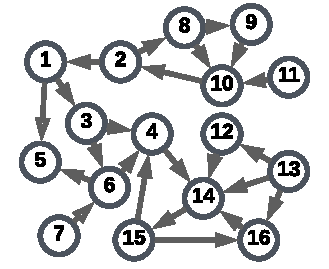
\includegraphics[width=0.23\linewidth]{out/about-frontier-11.pdf}
  }
  \subfigure[Marking initial affected vertices (DF)]{
    \label{fig:about-frontier-df2}
    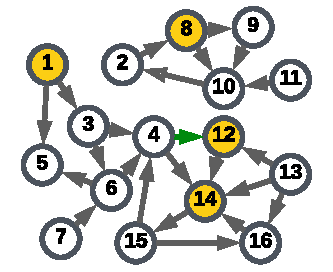
\includegraphics[width=0.23\linewidth]{out/about-frontier-32.pdf}
  }
  \subfigure[After first iteration (DF)]{
    \label{fig:about-frontier-df3}
    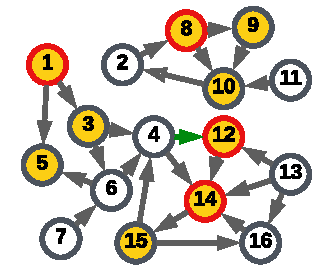
\includegraphics[width=0.23\linewidth]{out/about-frontier-33.pdf}
  }
  \subfigure[After second iteration (DF)]{
    \label{fig:about-frontier-df4}
    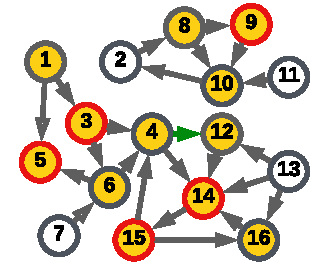
\includegraphics[width=0.23\linewidth]{out/about-frontier-34.pdf}
  } \\[2ex]
  \subfigure[Initial graph]{
    \label{fig:about-frontier-dfp1}
    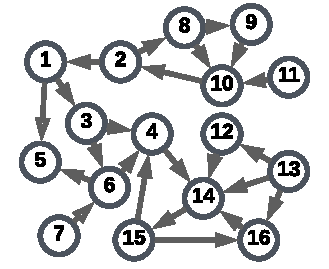
\includegraphics[width=0.23\linewidth]{out/about-frontier-11.pdf}
  }
  \subfigure[Marking initial affected vertices (DF-P)]{
    \label{fig:about-frontier-dfp2}
    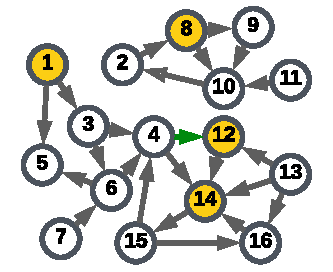
\includegraphics[width=0.23\linewidth]{out/about-frontier-32.pdf}
  }
  \subfigure[After first iteration (DF-P)]{
    \label{fig:about-frontier-dfp3}
    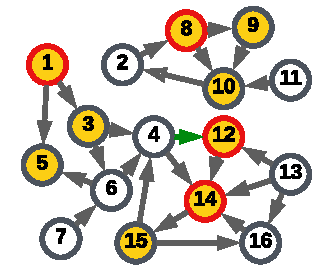
\includegraphics[width=0.23\linewidth]{out/about-frontier-33.pdf}
  }
  \subfigure[After second iteration (DF-P)]{
    \label{fig:about-frontier-dfp4}
    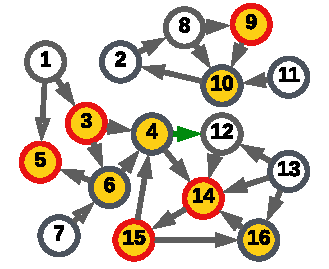
\includegraphics[width=0.23\linewidth]{out/about-frontier-44.pdf}
  } \\[2ex]
  \subfigure[Initial graph]{
    \label{fig:about-frontier-dt1}
    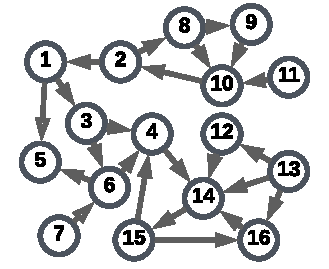
\includegraphics[width=0.23\linewidth]{out/about-frontier-11.pdf}
  }
  \subfigure[Marking affected vertices (DT)]{
    \label{fig:about-frontier-dt2}
    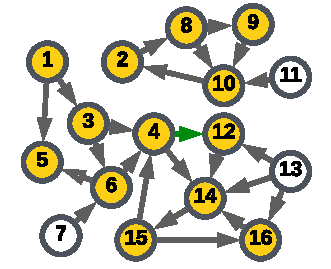
\includegraphics[width=0.23\linewidth]{out/about-frontier-22.pdf}
  }
  \subfigure[After first iteration (DT)]{
    \label{fig:about-frontier-dt3}
    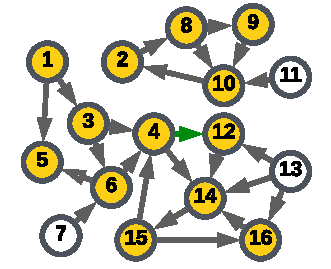
\includegraphics[width=0.23\linewidth]{out/about-frontier-22.pdf}
  }
  \subfigure[After second iteration (DT)]{
    \label{fig:about-frontier-dt4}
    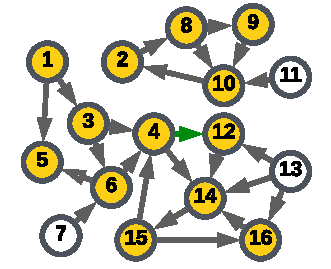
\includegraphics[width=0.23\linewidth]{out/about-frontier-22.pdf}
  } \\[-2ex]
  \caption{An example showcasing our improved \textit{Dynamic Frontier (DF)} and \textit{Dynamic Frontier with Pruning (DF-P)} approaches, in subfigures (a)-(d) and (e)-(h) respectively, in contrast to the \textit{Dynamic Traversal (DT)} approach, shown in subfigures (i)-(l).}
  \label{fig:about-frontier}
\end{figure*}

\ignore{An example showcasing our improved \textit{Dynamic Frontier (DF)} and \textit{Dynamic Frontier with Pruning (DF-P)} approaches. The initial graph has $16$ vertices and $23$ edges. The graph is updated with an edge insertion $(4, 12)$ and an edge deletion $(2, 1)$. Consequently, with DF and DF-P PageRank, the outgoing neighbors of vertices $2$ and $4$ (i.e., vertices $1$, $8$, $12$, and $14$) are marked as affected (shown with yellow fill). In the first iteration, when computing the ranks of these affected vertices, it is observed that the relative change in rank of vertices $1$, $8$, $12$, and $14$ exceeds the frontier tolerance $\tau_f$ (indicated with a red border). Therefore, their outgoing neighbors (i.e., vertices $3$, $5$, $9$, $10$, $14$, and $15$) are also marked as affected, with both DF and DF-P PageRank. In the second iteration, the relative rank change of vertices $3$, $5$, $9$, $14$, and $15$ surpasses the frontier tolerance $\tau_f$, resulting in their outgoing neighbors (i.e., vertices $4$, $6$, $10$, $15$, and $16$) being marked as affected. Additionally, with DF-P PageRank, vertices $1$, $8$, and $12$ are no longer marked as affected as their relative rank change falls below prune tolerance $\tau_p$. In the following iteration, the rankings of affected vertices are updated once more. If the rank change of each vertex falls within the iteration tolerance $\tau$, indicating convergence, the algorithm terminates. In contrast, the \textit{Dynamic Traversal (DT)} approach, marks all vertices reachable from $2$ and $4$ as affected. The ranks of this set of affected vertices are then updated in each iteration.}


\subsection{Our improved Dynamic Frontier approach}
\label{sec:frontier}

When a batch update $\Delta^{t-} \cup \Delta^{t+}$ is relatively small compared to the total number of edges $|E|$, it is anticipated that only a few vertices will experience rank changes. Our improved Dynamic Frontier approach addresses this scenario by employing an incremental process to identify affected vertices.\ignore{This helps minimize unnecessary computations, as vertices distant from the updated region of the graph are unlikely to experience rank changes until the ranks of their immediate in-neighbors change. In addition, we refrain from marking a vertex's neighbors as affected if the relative change in rank of the vertex is insignificant and is likely to have a minimal impact its neighbors ranks. We also avoid unnecessary computation of ranks of vertices that have likely settled, by no longer marking them as affected if the relative change in rank of the vertex is trivial.}


\subsubsection{Explanation of the approach}
\label{sec:frontier-explanation}

Consider a batch update consisting of edge deletions $(u, v) \in \Delta^{t-}$ and insertions $(u, v) \in \Delta^{t+}$. We first initialize the rank of each vertex to that obtained in the previous snapshot of the graph.

\paragraph{Initial marking of affected vertices:}

For each edge deletion/insertion $(u, v)$, we initially mark the outgoing neighbors of the vertex $u$ in the previous $G^{t-1}$ and current graph snapshot $G^t$ as affected.

\paragraph{Incremental expansion and contraction of the set of affected vertices upon change in rank of a given vertex:}

During PageRank computation, if the rank of any affected vertex $v$ changes in an iteration by a fraction greater than the \textit{frontier tolerance} $\tau_f$, we mark its outgoing neighbors as affected. This adjustment is made because a change in a vertex's rank is expected to influence the ranks of its outgoing neighbors. Additionally, if the relative change in rank of a vertex remains below the \textit{prune tolerance} $\tau_p$, the vertex is no longer marked as affected, as its rank may have converged. However, if the rank of such a vertex has not yet settled, it may be re-marked as affected by one of its in-neighbors. This process of marking and unmarking of vertices as affected continues in every iteration.


\subsubsection{A simple example}

Figure \ref{fig:about-frontier} illustrates an example of our improved Dynamic Frontier approach. Initially, as depicted in Figure \ref{fig:about-frontier-01}, the graph comprises $12$ vertices and $16$ edges. Subsequently, Figure \ref{fig:about-frontier-02} shows a batch update applied to the original graph, involving an edge insertion from vertex $6$ to $8$ and an edge deletion from vertex $2$ to $1$. Following the batch update, we proceed with the initial step of the Dynamic Frontier approach, marking outgoing neighbors of vertices $2$ and $6$ as affected, specifically vertices $1$, $3$, $8$, and $12$. These affected vertices are highlighted with a yellow fill. It is noteworthy that vertices $2$ and $6$ are not marked as affected. This is because changes in the out-degree of a vertex does not influence its PageRank score. Subsequently, we initiate the first iteration of the PageRank algorithm.

During the first iteration (refer to Figure \ref{fig:about-frontier-03}), the ranks of affected vertices are updated. It is observed that the relative change in rank of vertices $1$, $3$, $8$, and $12$ exceeds the frontier tolerance $\tau_f$. Such vertices are indicated with a red border in the figure. In response to this, we incrementally mark the outgoing neighbors of vertices $1$, $3$, $8$, and $12$ as affected, specifically vertices $4$, $5$, $7$, $9$, $11$, and $12$. Moreover, it is observed that the relative change in rank of vertices $1$, $3$, and $8$ remains below the prune tolerance $\tau_p$. As a result, these vertices are no longer marked as affected, as it is likely the ranks of such vertices have converged. This action effectively contracts the frontier of affected vertices. However, if the rank of such a vertex has not yet converged, it may be re-marked as affected by one of its in-neighbors.

In the second iteration, shown in Figure \ref{fig:about-frontier-04}, updates are made to the ranks of affected vertices once again. Here, it is observed that the relative change in rank of vertices $5$, $9$, $11$, and $12$ exceeds the frontier tolerance $\tau_f$. Consequently, we mark the outgoing neighbors of vertices $5$, $9$, $11$, and $12$ as affected, specifically vertices $6$, $10$, and $11$. Furthermore, vertices $4$, $5$, $7$, $9$, and $12$ are no longer marked as affected, as their relative rank change falls below the prune tolerance $\tau_p$. In the next iteration, the ranks of affected vertices are updated once more. If the change in rank of each vertex remains within the iteration tolerance $\tau$, the ranks of vertices have converged, and the algorithm terminates.




\ignore{\subsection{Synchronous vs Asynchronous implementation}}

\ignore{In a synchronous implementation, separate input and output rank vectors are used, ensuring deterministic results for parallel algorithms through vector swapping at the end of each iteration. In contrast, an asynchronous implementation utilizes a single rank vector, potentially achieving faster convergence and eliminating memory copies for unaffected vertices in dynamic approaches\ignore{, but introduces non-deterministic results in parallel algorithms}.}

\ignore{To assess synchronous and asynchronous implementations for Dynamic Frontier PageRank, both are tested on batch updates (purely edge insertions) ranging from $10^{-7}|E|$ to $0.1|E|$ for Static, Naive-dynamic, Dynamic Traversal, and Dynamic Frontier PageRank. Figure \ref{fig:approach-async} depicts the average relative runtime of asynchronous implementations compared to their synchronous counterparts. Based on the results, we use the asynchronous implementations of Naive-dynamic, Dynamic Traversal, and Dynamic Frontier PageRank --- as they are faster, especially for smaller batch sizes.\ignore{This is due to a somewhat faster convergence and the absence of copy overhead (for Dynamic Traversal and Dynamic Frontier approaches).}}




\subsection{Determination of Frontier tolerance ($\tau_f$)}
\label{sec:frontier-tolerance}

We first need to determine a suitable approach for frontier expansion, and an associate frontier tolerance $\tau_f$ value that allows us to minimize processed vertices, while limiting error to that of ranks obtained with Static PageRank using the same iteration tolerance $\tau$. For this, we experiment with three approaches. These include marking neighbors of a vertex as affected, based on change in rank of the vertex $\Delta r$, change in its contribution factor $\Delta r/d$, or relative change in its rank $\Delta r/r$. Here, $\Delta r$ is the rank change, $d$ is the out-degree, and $r$ is the vertex's \texttt{max} rank (the maximum of its previous and current rank values).

For $\Delta r$ and $\Delta r/d$, we adjust $\tau_f$ from $\tau$ to $\tau/10^5$; and for $\Delta r/r$, we adjust it from $0.1$ to $10^{-6}$. This is done on real world dynamic graphs, shown in Table \ref{tab:dataset}, with batch updates of size $10^{-5}|E_T|$. Outgoing neighbors are marked affected if the respective measure exceeds $\tau_f$. Figure \ref{fig:adjust-frontier} shows the mean speedup (with respect to Static PageRank) and rank error (compared to ranks obtained with reference Static PageRank) with each approach for frontier expansion. Results indicate that the $\Delta r/r$ approach with a $\tau_f$ of $10^{-6}$ performs best, while yielding lower error than Static PageRank.

\begin{figure*}[!hbt]
  \centering
  \subfigure[Speedup with varying Frontier tolerance $\tau_f$]{
    \label{fig:adjust-frontier--speedup}
    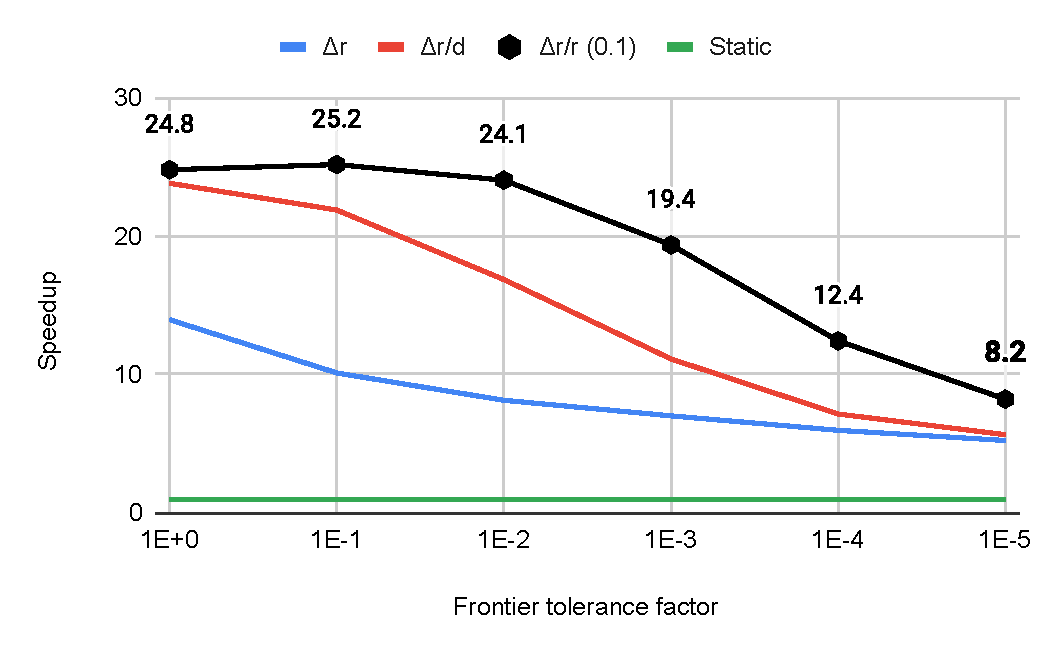
\includegraphics[width=0.48\linewidth]{out/adjust-frontier-speedup.pdf}
  }
  \subfigure[Error in ranks obtained with varying Frontier tolerance $\tau_f$]{
    \label{fig:adjust-frontier--error}
    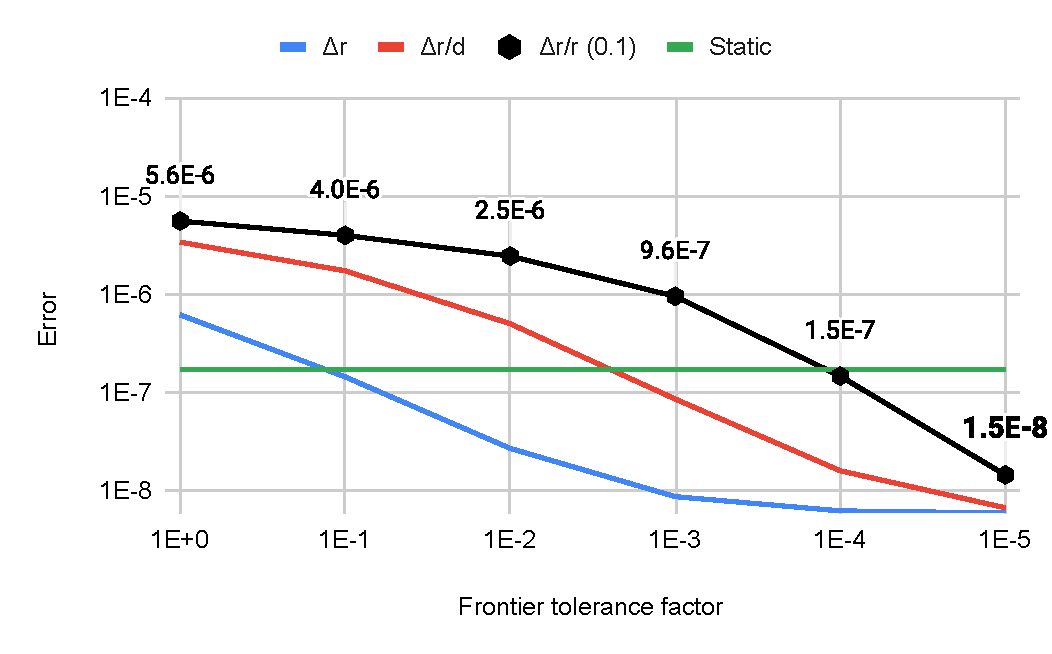
\includegraphics[width=0.48\linewidth]{out/adjust-frontier-error.pdf}
  } \\[-2ex]
  \caption{Average Speedup and Error in ranks obtained (with respect to ranks obtained with Reference Static PageRank) using \textit{Dynamic Frontier} approach, with frontier tolerance $\tau_f$ varying from $\tau$ to $\tau / 10^5$, on batch updates of size $10^{-7}|E|$ to $0.1|E|$. The figures indicate that increasing $\tau_f$ reduces runtime, but also increases the error. A Frontier tolerance $\tau_f$ of $\tau/10^4$ and $\tau/10^5$ obtain ranks with error lower than \textit{Static} PageRank, and are thus acceptable (we choose $\tau_f = \tau/10^5$ to be on the safe side).}
  \label{fig:adjust-frontier}
\end{figure*}

\begin{figure*}[!hbt]
  \centering
  \subfigure{
    \label{fig:adjust-prune--speedup}
    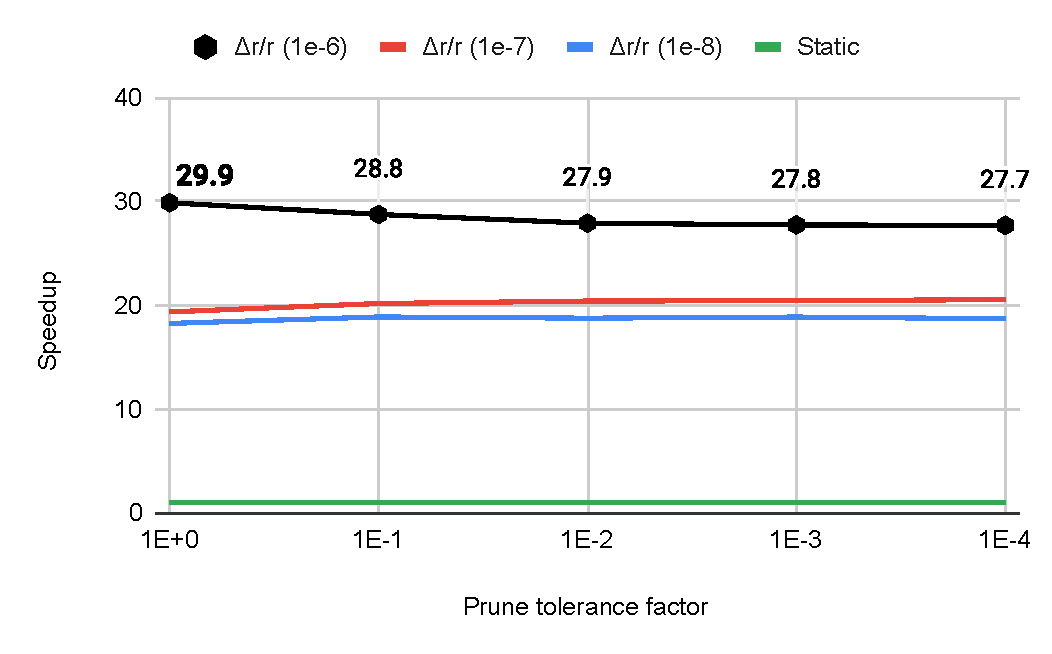
\includegraphics[width=0.48\linewidth]{out/adjust-prune-speedup.pdf}
  }
  \subfigure{
    \label{fig:adjust-prune--error}
    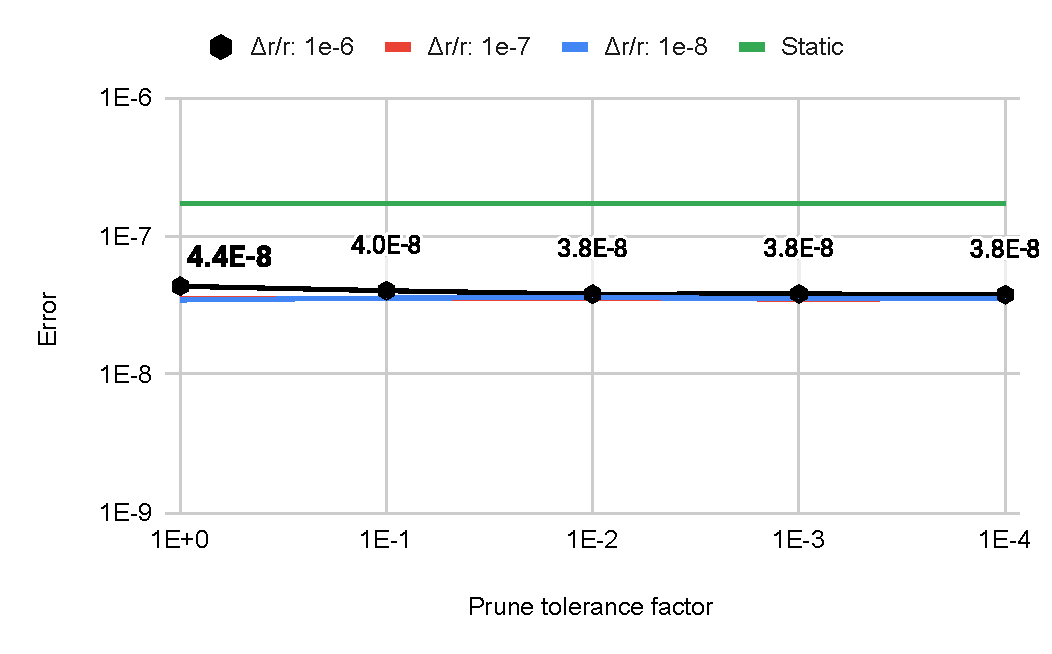
\includegraphics[width=0.48\linewidth]{out/adjust-prune-error.pdf}
  } \\[-2ex]
  \caption{Average Relative runtime with asynchronous implementations of \textit{Static}, \textit{Naive-dynamic}, \textit{Dynamic Traversal}, and \textit{Dynamic Frontier} approach compared to their respective synchronous implementations, on batch updates of size $10^{-7}|E|$ to $0.1|E|$ (right), and overall (left). The results indicate that asynchronous implementations are faster than synchronous ones, especially for smaller batch sizes. This is due to a somewhat faster convergence and the absence of copy overhead (for \textit{Dynamic Traversal} and \textit{Dynamic Frontier} approaches).}
  \label{fig:adjust-prune}
\end{figure*}

\begin{algorithm}[!hbt]
\caption{Our parallel Dynamic Frontier (DF) PageRank.}
\label{alg:frontier}
\begin{algorithmic}[1]
\Require{$G^{t-1}, G^t$: Previous, current input graph}
\Require{$\Delta^{t-}, \Delta^{t+}$: Edge deletions and insertions (input)}
\Require{$R^{t-1}, R$: Previous, current rank vector}
\Ensure{$\Delta r$: Change in rank of a vertex}
\Ensure{$\Delta R$: $L\infty$-norm between previous and current ranks}
\Ensure{$\tau, \tau_f, \tau_p$: Iteration, frontier, prune tolerance}
\Ensure{$\alpha$: Damping factor}

\Statex

\Function{dynamicFrontier}{$G^{t-1}, G^t, \Delta^{t-}, \Delta^{t+}, R^{t-1}$}
  \State $R \gets R^{t-1}$ \label{alg:frontier--initialize}
  \State $\rhd$ Mark initial affected
  \ForAll{$(u, v) \in \Delta^{t-} \cup \Delta^{t+} \textbf{in parallel}$} \label{alg:frontier--mark-begin}
    \ForAll{$v' \in (G^{t-1} \cup G^t).out(u)$}
    \State Mark $v'$ as affected
    \EndFor
  \EndFor \label{alg:frontier--mark-end}
  \ForAll{$i \in [0 .. MAX\_ITERATIONS)$} \label{alg:frontier--compute-begin}
    \State $\Delta R \gets 0$
    \ForAll{affected $v \in V^t$ \textbf{in parallel}}
      \State $r \gets (1 - \alpha)/|V^t|$
      \ForAll{$u \in G^t.in(v)$}
        \State $r \gets r + \alpha * R[u] / |G^t.out(u)|$
      \EndFor
      \State $\Delta r \gets |r - R[v]|$ \textbf{;} $\Delta R \gets \max(\Delta R, \Delta r)$
      \State $\rhd$ Prune $v$ if its relative rank change is small
      \If{$\Delta r / \max(r, R[v]) \leq \tau_p$}
        \State Mark $v$ as not affected
      \EndIf
      \State $\rhd$ Expand frontier if relative rank change is large
      \If{$\Delta r / \max(r, R[v]) > \tau_f$} \label{alg:frontier--remark-begin}
        \ForAll{$v' \in G^t.out(v)$}
          \State Mark $v'$ as affected
        \EndFor
      \EndIf \label{alg:frontier--remark-end}
      \State $\rhd$ Update rank of $v$
      \State $R[v] \gets r$
    \EndFor
    \State $\rhd$ Ranks converged?
    \If{$\Delta R \le \tau$} \textbf{break}
    \EndIf
  \EndFor \label{alg:frontier--compute-end}
  \State \ReturnInline{$R$} \label{alg:frontier--return}
\EndFunction
\end{algorithmic}
\end{algorithm}




%% Requires (parameters):
% G(V, E): a directed unweighted graph
% R: initial ranks (1/N for static)

%% Parameter values:
% MAX\_ITERATIONS = 500
% DAMPING\_FACTOR = 0.85
% TOLERANCE = 10^-10





\subsection{Determination of Prune tolerance ($\tau_p$)}
\label{sec:prune-tolerance}

We now measure a suitable value for prune tolerance $\tau_p$ for the best approach of frontier expansion $\Delta r/r$ with a frontier tolerance $\tau_f$ of $10^{-6}$, as identified in Section \ref{sec:frontier-tolerance}. For this, we adjust $\tau_p$ from $\tau_f$ to $\tau_f/10^5$. In addition, we also experiment with $\tau_f$ of $10^{-7}$ and $10^{-8}$ to be on the safe side. This is done on real world graphs, with batch updates of size $10^{-5}|E_T|$ (as earlier). A vertex is marked as unaffected, if its relative rank change $\Delta r/r$ lies within $\tau_p$.

Figure \ref{fig:adjust-prune} illustrates the mean speedup (compared to Static PageRank) and error in ranks obtained (with respect to ranks from reference Static PageRank, see Section \ref{sec:measurement}) with each $\tau_f$ for frontier expansion. The figure indicates that the $\Delta r/r$ approach with a $\tau_f$ of $10^{-6}$ and a $\tau_p$ of $\tau_f = 10^{-6}$ performs the best, while obtaining ranks with lower error than Static PageRank.




\subsection{Our DF-PageRank implementation}

Algorithm \ref{alg:frontier} shows the implementation of our improved Dynamic Frontier (DF) PageRank approach. It takes as input the previous $G^{t-1}$ and current $G^t$ snapshot of the graph, edge deletions $\Delta^{t-}$ and insertions $\Delta^{t+}$ in the batch update, the previous rank vector $R^{t-1}$, and returns as output, the updated ranks $R$.

The algorithm begins by initializing the current rank vector $R$ with the previous rank vector $R^{t-1}$ (line \ref{alg:frontier--initialize}), and marking the initially affected vertices based on edge deletions $\Delta^{t-}$ and insertions $\Delta^{t+}$ in parallel (lines \ref{alg:frontier--mark-begin}-\ref{alg:frontier--mark-end}). It then iteratively computes the rank $R[v]$ for each affected vertex $v$ (lines \ref{alg:frontier--compute-begin}-\ref{alg:frontier--compute-end}). This computation is performed in parallel, considering the incoming edges $G^t.in(v)$. The algorithm checks if the relative change in rank $\Delta r / \max(r, R[v])$ exceeds the frontier tolerance $\tau_f$, marking out-neighbor vertices as affected if so. Additionally, if the relative change in rank lies within the prune tolerance $\tau_p$, the vertex $v$ is marked as not affected. The iteration continues until either the maximum change in ranks $\Delta R$ falls below the iteration tolerance $\tau$, or the maximum number of iterations $MAX\_ITERATIONS$ is reached. Finally, the algorithm returns the final rank vector $R$ (line \ref{alg:frontier--return}).

In a push-based approach for PageRank computation, each thread calculates and sums the outgoing PageRank contribution of its vertex to its neighbors, necessitating atomic updates. In contrast, with a pull-based approach, each vertex's rank is updated through a single write by a thread \cite{verstraaten2015quantifying}. We find this to be more efficient and employ it for all implementations. Furthermore, we employ an asynchronous implementation of DF-PageRank, using a single rank vector, for potentially faster convergence and elimination of memory copies for unaffected vertices. This, based on our previous research \cite{sahu2024incrementally}, outperforms synchronous implementations, especially with smaller batch sizes. Additionally, we utilize asynchronous implementations of Naive-dynamic (ND) and Dynamic Traversal (DT) PageRank.




% Dynamic Frontier (DF) approach
% Adjusting tolerance, Frontier tolerance, Mark DelRank / DelContrib
% Dynamic Frontier optimizations
% Edge-balanced approach (Chunk size)


\section{Evaluation}
\label{sec:evaluation}
\subsection{Experimental Setup}
\label{sec:setup}

\subsubsection{System used}

Experiments are performed on a system featuring an AMD EPYC-7742 processor with $64$ cores, operating at a frequency of $2.25$ GHz. Each core is equipped with a $4$ MB L1 cache, a $32$ MB L2 cache, and shares a $256$ MB L3 cache. The server is set up with $512$ GB of DDR4 system memory and runs on Ubuntu $20.04$.


\subsubsection{Configuration}

We utilize 32-bit integers for vertex IDs and 64-bit floating-point numbers for vertex ranks. Affected vertices are represented using an 8-bit integer vector. The rank computation employs OpenMP's \textit{dynamic schedule} with a chunk size of $2048$, facilitating dynamic workload balancing among threads. We use a damping factor of $\alpha = 0.85$ \cite{rank-langville06}, with an iteration tolerance of $\tau = 10^{-10}$ using the $L_\infty$-norm \cite{rank-dubey22, rank-plimpton11}. The maximum number of iterations (\texttt{MAX\_ITERATIONS}) is limited to $500$ \cite{nvgraph}. All experiments are conducted with $64$ threads to match the number of cores available on the system, unless specified otherwise. Compilation is carried out using GCC $9.4$ and OpenMP $5.0$.


\subsubsection{Dataset}

We use the largest five temporal networks from the Stanford Large Network Dataset Collection \cite{snapnets}, as detailed in Table \ref{tab:dataset}. The number of vertices in these graphs range from $X$ million to $X$ million, with temporal edge counts spanning from $X$ million to $X$ billion, and static edge counts spanning from $X$ million to $X$ billion. For the experiment in Section $X$, we use four classes of static graphs (as batch update are randomly generated, with uniform probability for selection of any vertex as the endpoint of an edge to be inserted or deleted), sourced from the \textit{SuiteSparse Matrix Collection} \cite{suite19}, as detailed in Table \ref{tab:dataset}. The number of vertices in these graphs range from $3.07$ million to $214$ million, with edge counts spanning from $37.4$ million to $1.98$ billion. To address the impact of dead ends (vertices lacking out-links), a global teleport rank computation is needed in each iteration. We mitigate this overhead by adding self-loops to all vertices in the graph \cite{rank-andersen07, rank-langville06}.

\begin{table}[hbtp]
  \centering
  \caption{List of 5 real-world dynamic graphs\ignore{, i.e., temporal networks}, obtained from the Stanford Large Network Dataset Collection \cite{snapnets}. Here, $|V|$ is the number of vertices, $|E_T|$ the number of temporal edges\ignore{(includes duplicate edges)}, and $|E|$ the number of static edges (with no duplicates).\ignore{, and $\Gamma_G$ is the Gini coefficient of PageRank distribution. In the table, B refers to a billion, M refers to a million and K refers a thousand.}}
  \label{tab:dataset}
  \begin{tabular}{|c||c|c|c|c|}
    \toprule
    \textbf{Graph} &
    \textbf{\textbf{$|V|$}} &
    \textbf{\textbf{$|E_T|$}} &
    \textbf{\textbf{$|E|$}} \\
    \midrule
    sx-mathoverflow & 24.8K & 507K & 240K \\ \hline
    sx-askubuntu & 159K & 964K & 597K \\ \hline
    sx-superuser & 194K & 1.44M & 925K \\ \hline
    wiki-talk-temporal & 1.14M & 7.83M & 3.31M \\ \hline
    sx-stackoverflow & 2.60M & 63.4M & 36.2M \\ \hline
  \bottomrule
  \end{tabular}
\end{table}



\subsubsection{Batch Generation}
\label{sec:batch-generation}

For each base (static) graph from the dataset, we generate a random batch update, consisting of purely edge insertions, purely edge deletions, or an $80\% : 20\%$ mix of edge insertions and deletions to mimic realistic batch updates. The set of edges for insertion is prepared by selecting vertex pairs with equal probability. To construct the set of edge deletions, we delete each existing edge with a uniform probability. For simplicity, we ensure that no new vertices are added to or removed from the graph. The batch size is measured as a fraction of edges in the original graph, and is varied from $10^{-7}$ to $0.1$ (i.e., $10^{-7}|E|$ to $0.1|E|$), with multiple batches generated for each size (for averaging). Along with each batch update, self-loops are added to all vertices.


\subsubsection{Measurement}
\label{sec:measurement}

We measure the time taken by each approach on the updated graph entirely, including any preprocessing costs and convergence detection time, while excluding time dedicated to memory allocation and deallocation. The mean time for a specific method at a given batch size is calculated as the geometric mean across various input graphs. Consequently, the average speedup is determined as the ratio of these mean times. Additionally, we gauge the error/accuracy of a given approach by assessing the $L1$-norm \cite{ohsaka2015efficient} of the ranks in comparison to ranks obtained from a reference Static PageRank run on the updated graph with an extremely low iteration tolerance of $\tau = 10^{-100}$ (limited to $500$ iterations).

\begin{figure*}[!hbt]
  \centering
  \subfigure[]{
    \label{fig:temporal-all--runtime}
    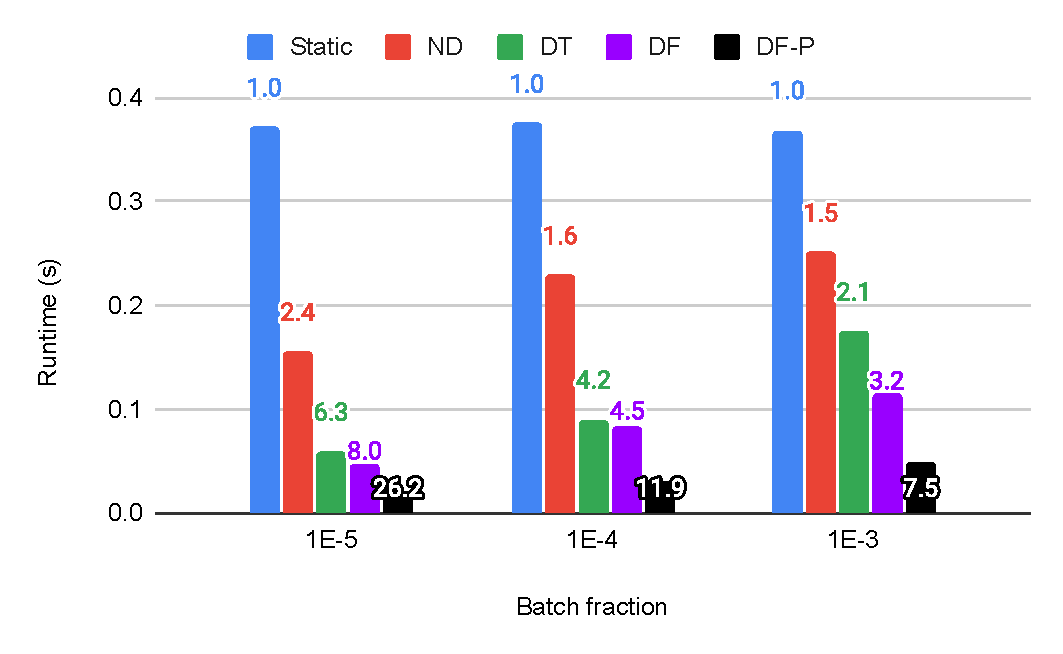
\includegraphics[width=0.48\linewidth]{out/temporal-all-runtime.pdf}
  }
  \subfigure{
    \label{fig:temporal-all--error}
    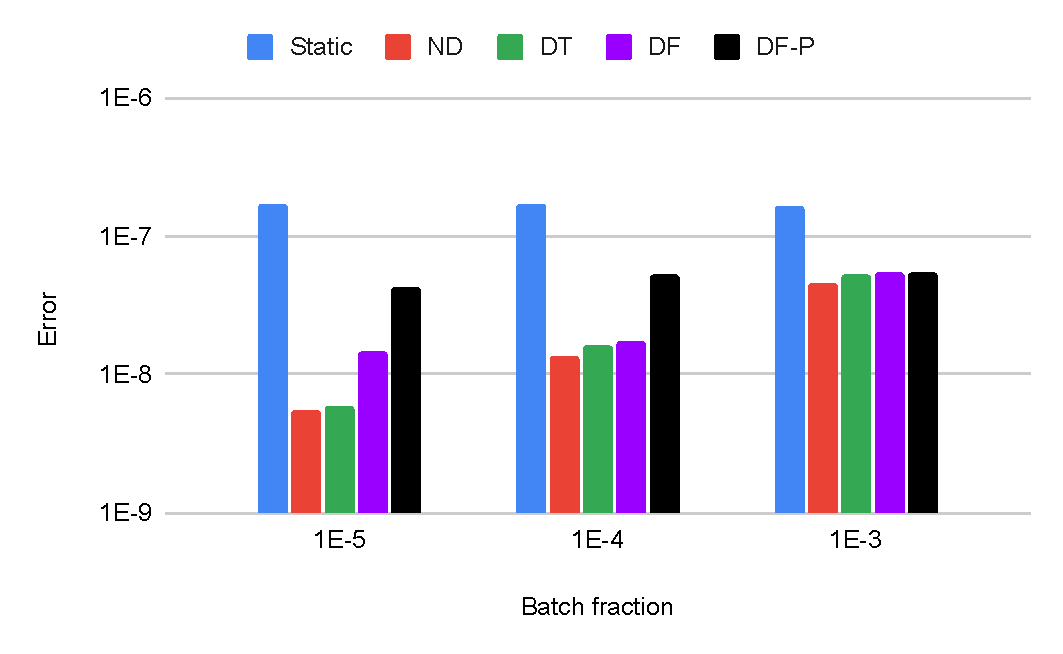
\includegraphics[width=0.48\linewidth]{out/temporal-all-error.pdf}
  } \\[-4ex]
  \caption{Overall Runtime and Error in ranks obtained with \textit{Static}, \textit{Naive-dynamic (ND)}, \textit{Dynamic Traversal (DT)}, and our improved \textit{Dynamic Frontier (DF)} PageRank on real world dynamic graphs, with batch updates of size $10^{-5}|E|$ to $10^{-3}|E|$. In (a), the speedup of each approach with respect to Static PageRank is labeled.}
  \label{fig:temporal-all}
\end{figure*}

\begin{figure*}[!hbt]
  \centering
  \subfigure{
    \label{fig:temporal-batch5--runtime}
    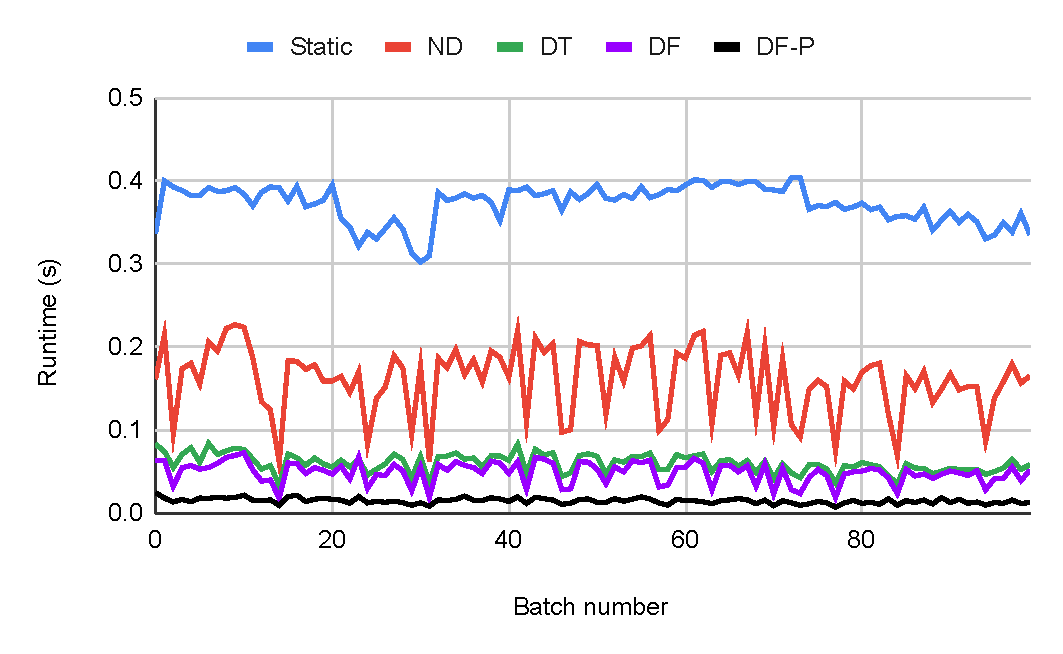
\includegraphics[width=0.48\linewidth]{out/temporal-batch5-runtime.pdf}
  }
  \subfigure{
    \label{fig:temporal-batch5--error}
    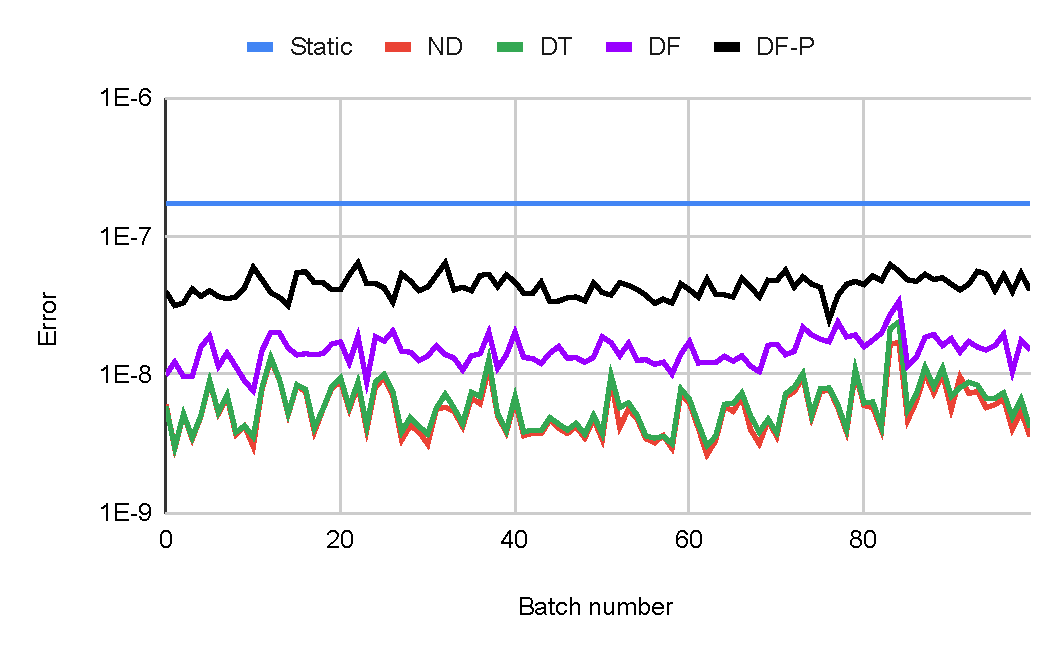
\includegraphics[width=0.48\linewidth]{out/temporal-batch5-error.pdf}
  } \\[-2ex]
  \caption{Average Relative runtime with asynchronous implementations of \textit{Static}, \textit{Naive-dynamic}, \textit{Dynamic Traversal}, and \textit{Dynamic Frontier} approach compared to their respective synchronous implementations, on batch updates of size $10^{-7}|E|$ to $0.1|E|$ (right), and overall (left). The results indicate that asynchronous implementations are faster than synchronous ones, especially for smaller batch sizes. This is due to a somewhat faster convergence and the absence of copy overhead (for \textit{Dynamic Traversal} and \textit{Dynamic Frontier} approaches).}
  \label{fig:temporal-batch5}
\end{figure*}

\begin{figure*}[!hbt]
  \centering
  \subfigure{
    \label{fig:temporal-batch4--runtime}
    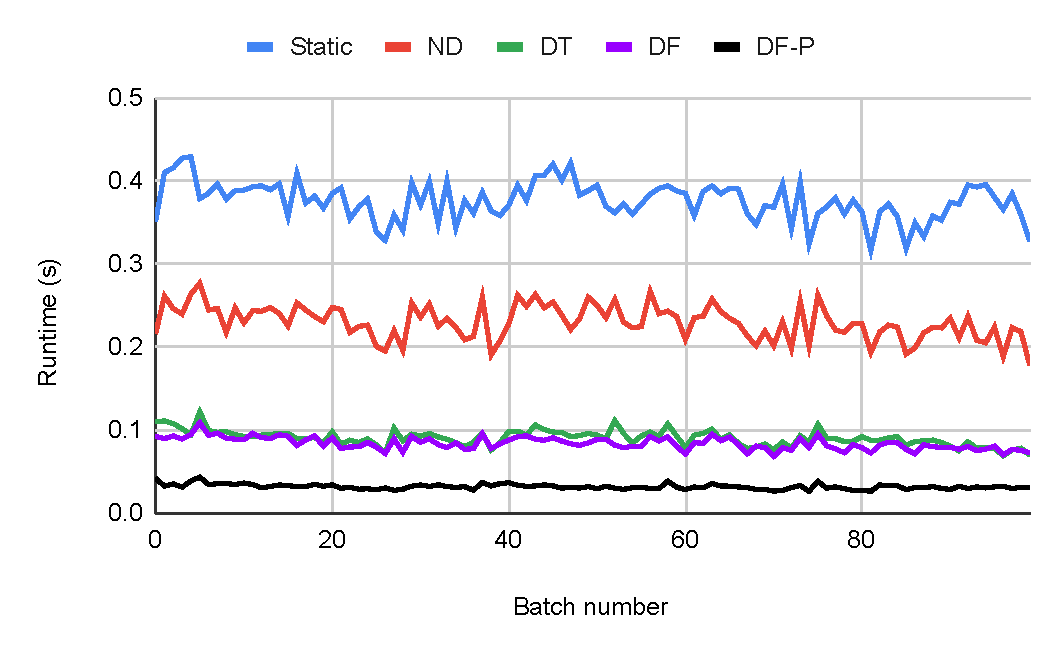
\includegraphics[width=0.48\linewidth]{out/temporal-batch4-runtime.pdf}
  }
  \subfigure{
    \label{fig:temporal-batch4--error}
    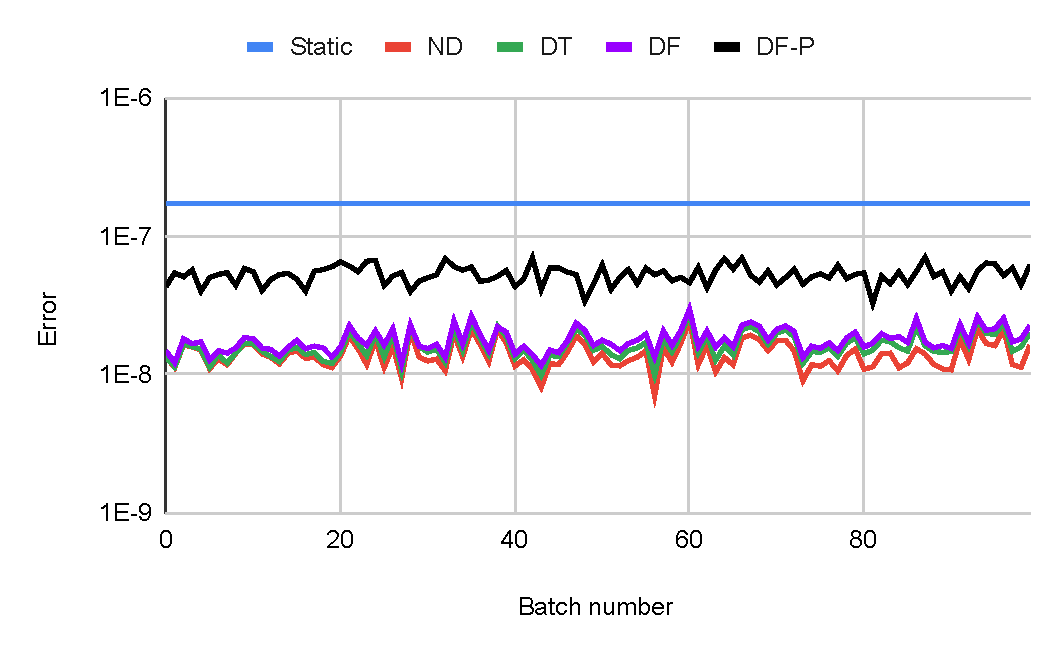
\includegraphics[width=0.48\linewidth]{out/temporal-batch4-error.pdf}
  } \\[-2ex]
  \caption{Average Relative runtime with asynchronous implementations of \textit{Static}, \textit{Naive-dynamic}, \textit{Dynamic Traversal}, and \textit{Dynamic Frontier} approach compared to their respective synchronous implementations, on batch updates of size $10^{-7}|E|$ to $0.1|E|$ (right), and overall (left). The results indicate that asynchronous implementations are faster than synchronous ones, especially for smaller batch sizes. This is due to a somewhat faster convergence and the absence of copy overhead (for \textit{Dynamic Traversal} and \textit{Dynamic Frontier} approaches).}
  \label{fig:temporal-batch4}
\end{figure*}

\begin{figure*}[!hbt]
  \centering
  \subfigure{
    \label{fig:temporal-batch3--runtime}
    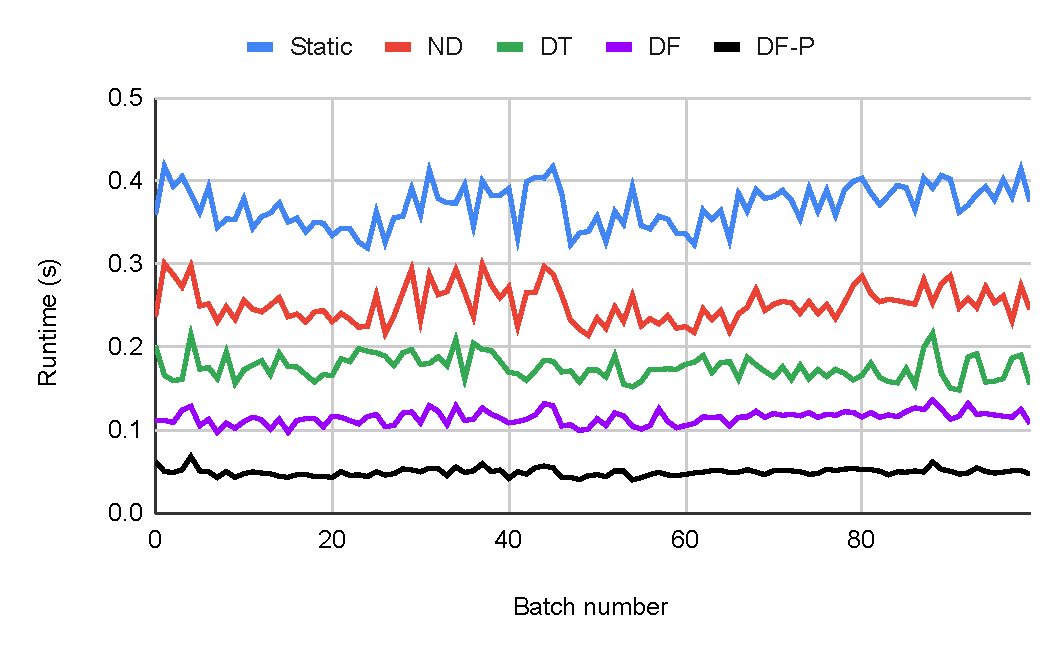
\includegraphics[width=0.48\linewidth]{out/temporal-batch3-runtime.pdf}
  }
  \subfigure{
    \label{fig:temporal-batch3--error}
    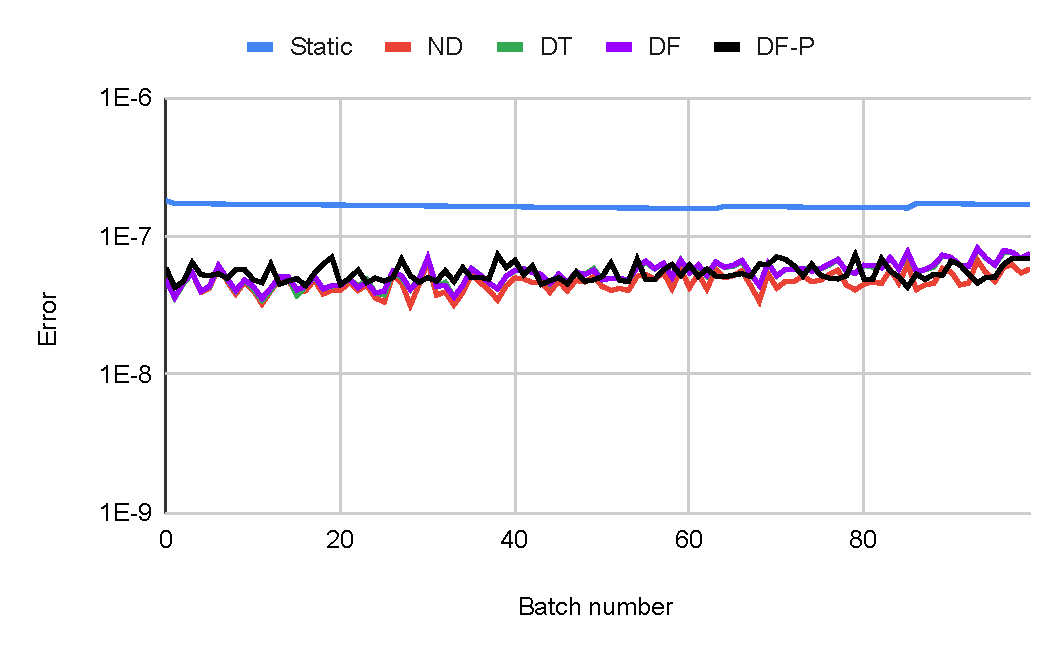
\includegraphics[width=0.48\linewidth]{out/temporal-batch3-error.pdf}
  } \\[-2ex]
  \caption{Average Relative runtime with asynchronous implementations of \textit{Static}, \textit{Naive-dynamic}, \textit{Dynamic Traversal}, and \textit{Dynamic Frontier} approach compared to their respective synchronous implementations, on batch updates of size $10^{-7}|E|$ to $0.1|E|$ (right), and overall (left). The results indicate that asynchronous implementations are faster than synchronous ones, especially for smaller batch sizes. This is due to a somewhat faster convergence and the absence of copy overhead (for \textit{Dynamic Traversal} and \textit{Dynamic Frontier} approaches).}
  \label{fig:temporal-batch3}
\end{figure*}

\begin{figure*}[!hbt]
  \centering
  \subfigure{
    \label{fig:temporal-large--runtime}
    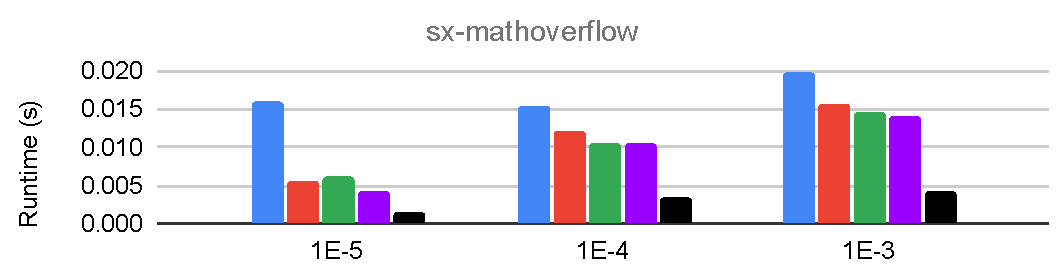
\includegraphics[width=0.48\linewidth]{out/temporal-large-runtime-sx-mathoverflow.pdf}
  }
  \subfigure{
    \label{fig:temporal-large--error}
    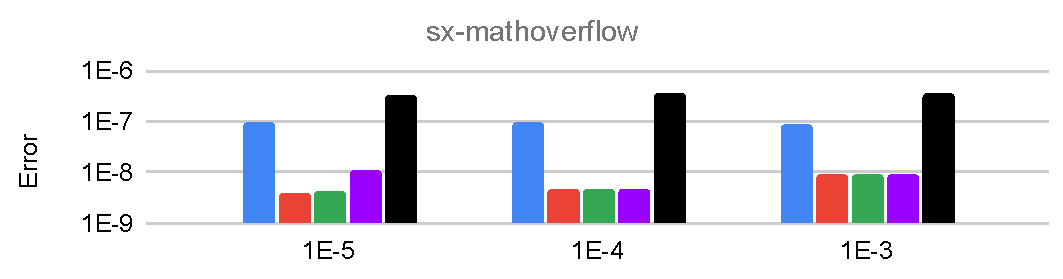
\includegraphics[width=0.48\linewidth]{out/temporal-large-error-sx-mathoverflow.pdf}
  }
  \subfigure{
    \label{fig:temporal-large--runtime}
    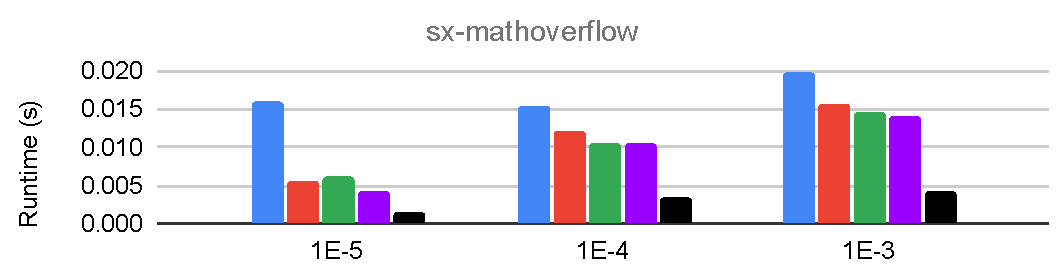
\includegraphics[width=0.48\linewidth]{out/temporal-large-runtime-sx-mathoverflow.pdf}
  }
  \subfigure{
    \label{fig:temporal-large--error}
    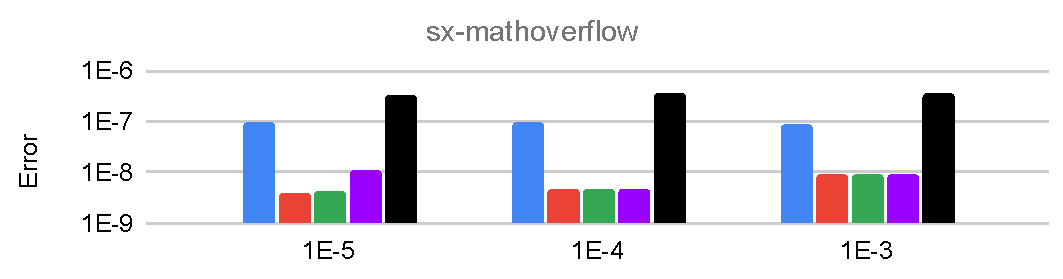
\includegraphics[width=0.48\linewidth]{out/temporal-large-error-sx-mathoverflow.pdf}
  }
  \subfigure{
    \label{fig:temporal-large--runtime}
    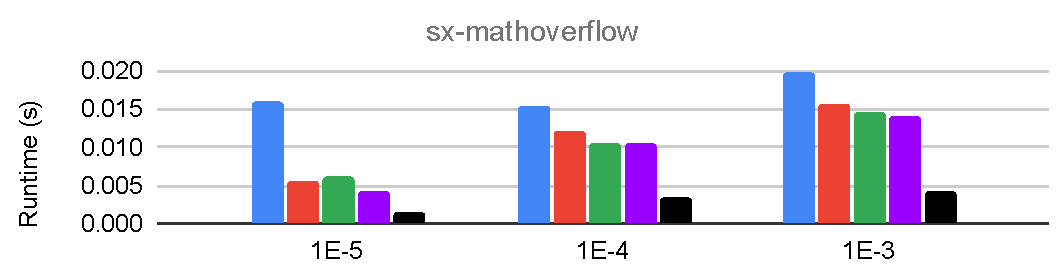
\includegraphics[width=0.48\linewidth]{out/temporal-large-runtime-sx-mathoverflow.pdf}
  }
  \subfigure{
    \label{fig:temporal-large--error}
    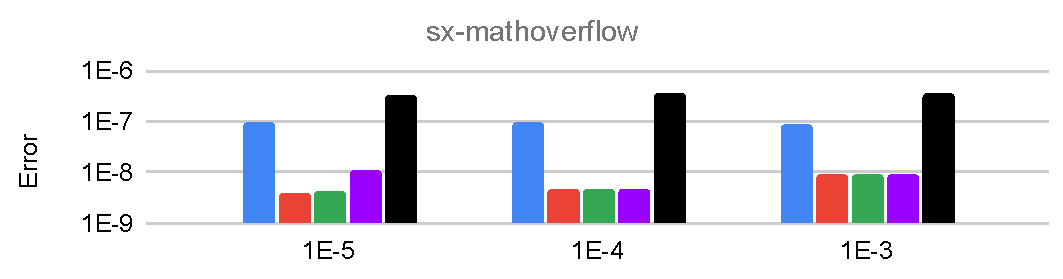
\includegraphics[width=0.48\linewidth]{out/temporal-large-error-sx-mathoverflow.pdf}
  }
  \subfigure{
    \label{fig:temporal-large--runtime}
    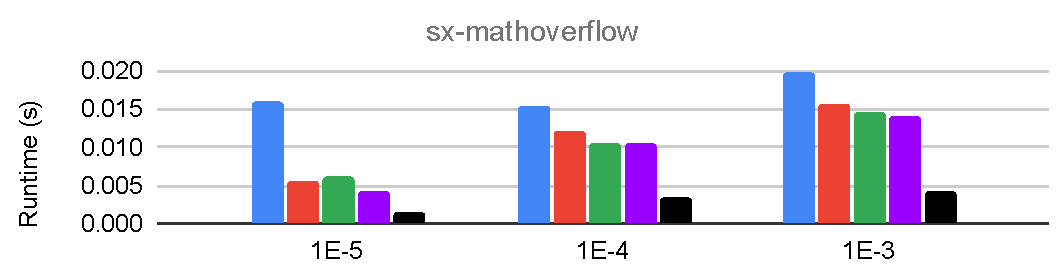
\includegraphics[width=0.48\linewidth]{out/temporal-large-runtime-sx-mathoverflow.pdf}
  }
  \subfigure{
    \label{fig:temporal-large--error}
    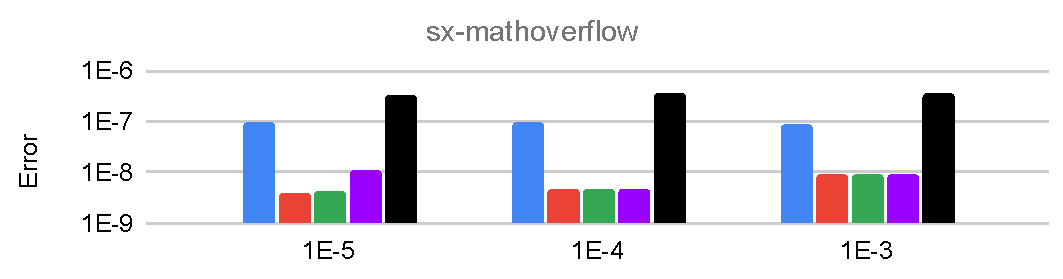
\includegraphics[width=0.48\linewidth]{out/temporal-large-error-sx-mathoverflow.pdf}
  }
  \subfigure{
    \label{fig:temporal-large--runtime}
    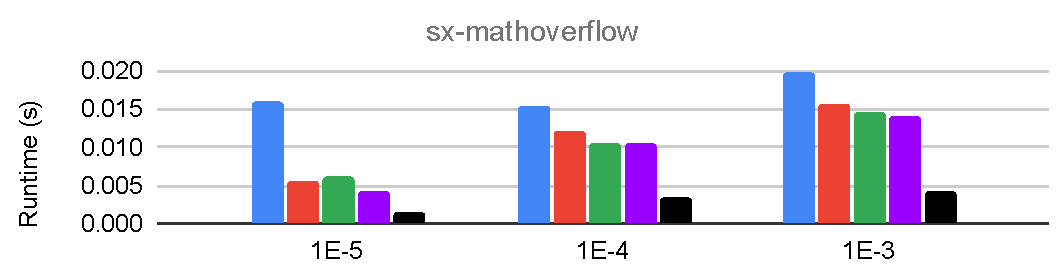
\includegraphics[width=0.48\linewidth]{out/temporal-large-runtime-sx-mathoverflow.pdf}
  }
  \subfigure{
    \label{fig:temporal-large--error}
    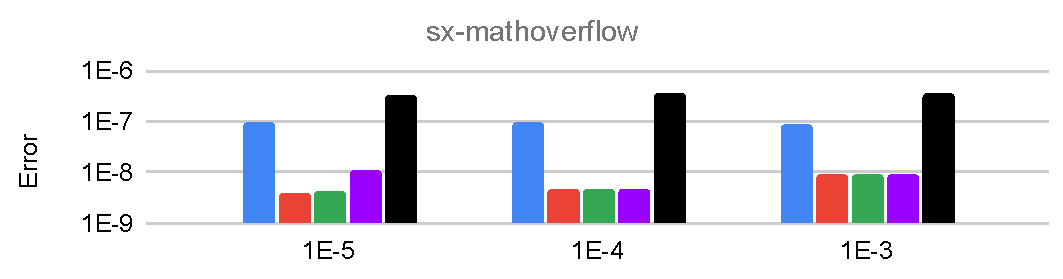
\includegraphics[width=0.48\linewidth]{out/temporal-large-error-sx-mathoverflow.pdf}
  } \\[-2ex]
  \caption{Average Relative runtime with asynchronous implementations of \textit{Static}, \textit{Naive-dynamic}, \textit{Dynamic Traversal}, and \textit{Dynamic Frontier} approach compared to their respective synchronous implementations, on batch updates of size $10^{-7}|E|$ to $0.1|E|$ (right), and overall (left). The results indicate that asynchronous implementations are faster than synchronous ones, especially for smaller batch sizes. This is due to a somewhat faster convergence and the absence of copy overhead (for \textit{Dynamic Traversal} and \textit{Dynamic Frontier} approaches).}
  \label{fig:temporal-large}
\end{figure*}

% \begin{figure*}[hbtp]
  \centering
  % \includegraphics[width=0.44\linewidth]{out/8020-runtime-key.pdf}
  \subfigure[Overall result]{
    \label{fig:8020-runtime--mean}
    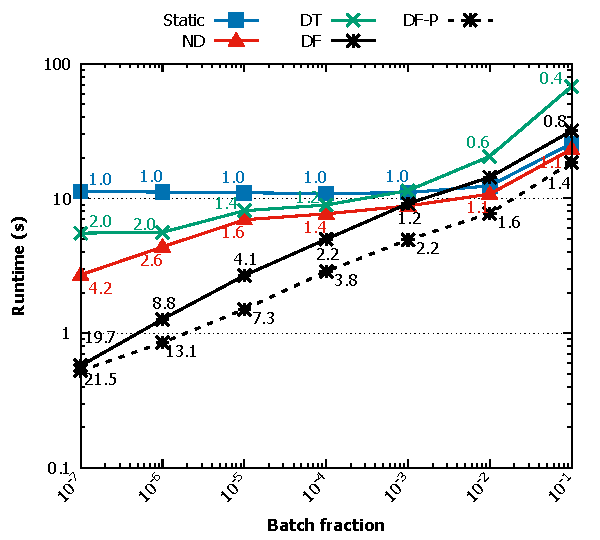
\includegraphics[width=0.38\linewidth]{out/8020-runtime-mean.pdf}
  }
  \subfigure[Results on each graph]{
    \label{fig:8020-runtime--all}
    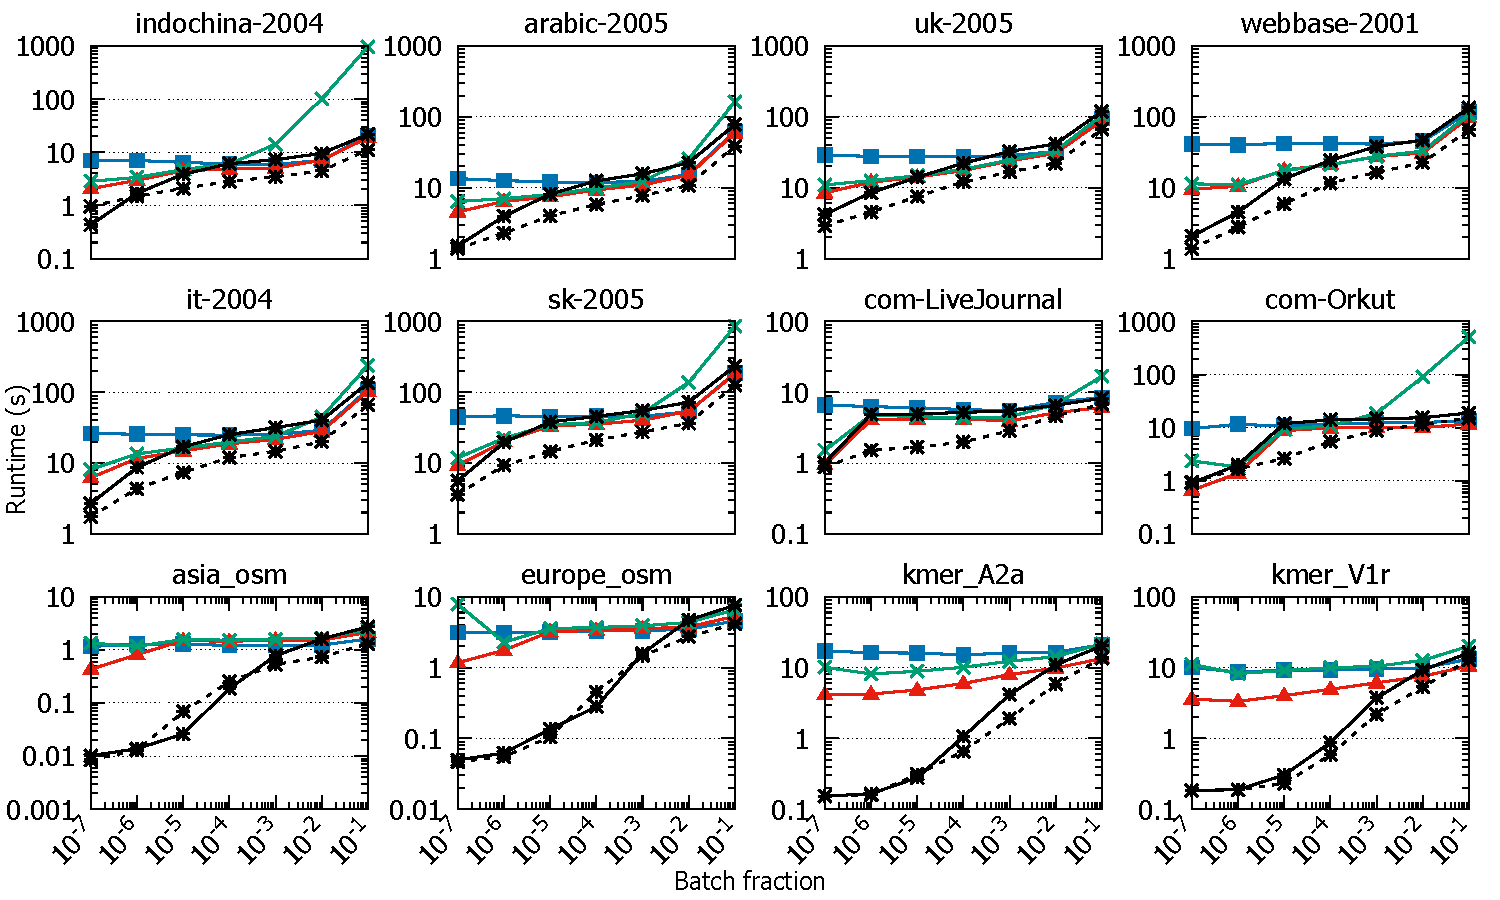
\includegraphics[width=0.58\linewidth]{out/8020-runtime-all.pdf}
  } \\[-1ex]
  \caption{Runtime (logarithmic scale) of \textit{Static}, \textit{Naive-dynamic}, \textit{Dynamic Traversal}, and \textit{Dynamic Frontier} PageRank with batch updates increasing from $10^{-7} |E|$ to $0.1 |E|$, in multiples of $10$ (logarithmic scale). The updates include $80\%$ edge insertions and $20\%$ edge deletions, simulating realistic changes upon a dynamic graph. The figure on the right illustrates the runtime of each approach for each graph in the dataset, while the figure of the left presents overall runtimes (using geometric mean for consistent scaling across graphs).}
  \label{fig:8020-runtime}
\end{figure*}

% \begin{figure*}[hbtp]
  \centering
  % \includegraphics[width=0.44\linewidth]{out/8020-speedup-key.pdf}
  \subfigure[Overall result]{
    \label{fig:8020-speedup--mean}
    \includegraphics[width=0.38\linewidth]{out/8020-speedup-mean.pdf}
  }
  \subfigure[Results on each graph]{
    \label{fig:8020-speedup--all}
    \includegraphics[width=0.58\linewidth]{out/8020-speedup-all.pdf}
  } \\[-1ex]
  \caption{Speedup of \textit{Dynamic Frontier} PageRank with respect to \textit{Static}, \textit{Naive-dynamic}, and \textit{Dynamic Traversal} PageRank on batch updates of size $10^{-7} |E|$ to $0.1 |E|$ (logarithmic scale), with $80\%$ edge insertions and $20\%$ edge deletions --- representing a realistic batch update upon a dynamic graph. The figure on the right shows the speedup of \textit{Dynamic Frontier} PageRank, with respect to each approach, for each graph in the dataset --- while the figure of the left highlights the overall speedup.}
  \label{fig:8020-speedup}
\end{figure*}

% \begin{figure*}[hbtp]
  \centering
  \subfigure[Overall result]{
    \label{fig:8020-error--mean}
    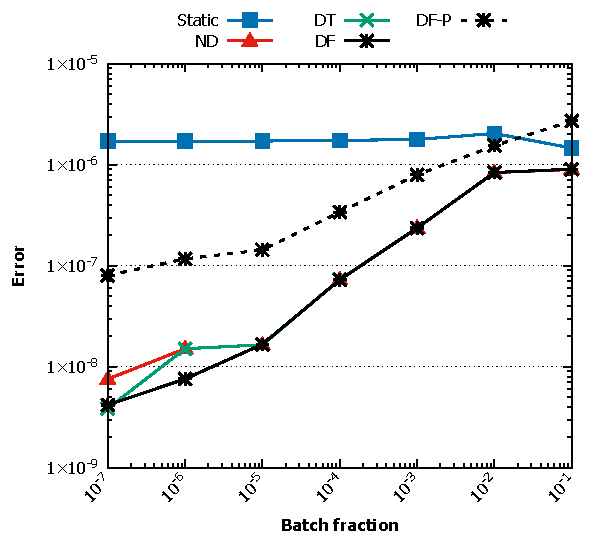
\includegraphics[width=0.38\linewidth]{out/8020-error-mean.pdf}
  }
  \subfigure[Results on each graph]{
    \label{fig:8020-error--all}
    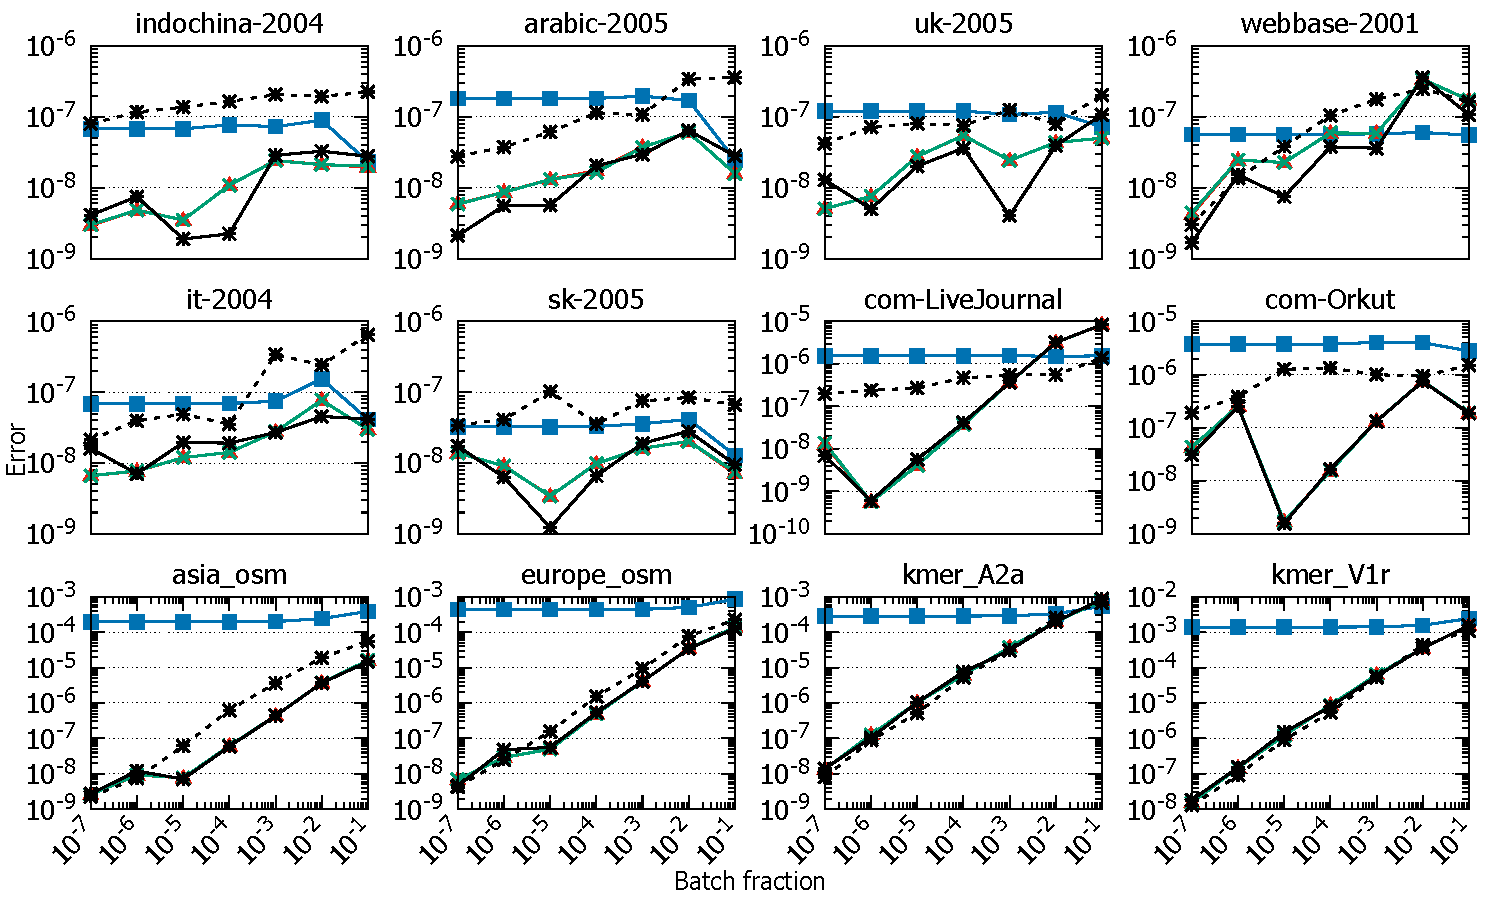
\includegraphics[width=0.58\linewidth]{out/8020-error-all.pdf}
  } \\[-1ex]
  \caption{Error comparison of \textit{Static}, \textit{Naive-dynamic (ND)}, \textit{Dynamic Traversal (DT)}, our improved \textit{Dynamic Frontier (DF)}, and \textit{Dynamic Frontier with Pruning (DF-P)} PageRank on large (static) graphs with generated random batch updates, relative to a Reference Static PageRank (see Section \ref{sec:measurement}), using $L1$-norm. The size of batch updates range from $10^{-7} |E|$ to $0.1 |E|$ in multiples of $10$ (logarithmic scale), consisting of $80\%$ edge insertions and $20\%$ edge deletions to simulate realistic dynamic graph updates. The right subfigure depicts the error for each approach in relation to each graph, while the left subfigure showcases overall errors using geometric mean for consistent scaling across graphs.}
  \label{fig:8020-error}
\end{figure*}

% \begin{figure}[!hbt]
  \centering
  \subfigure{
    \label{fig:measure-affected--batch}
    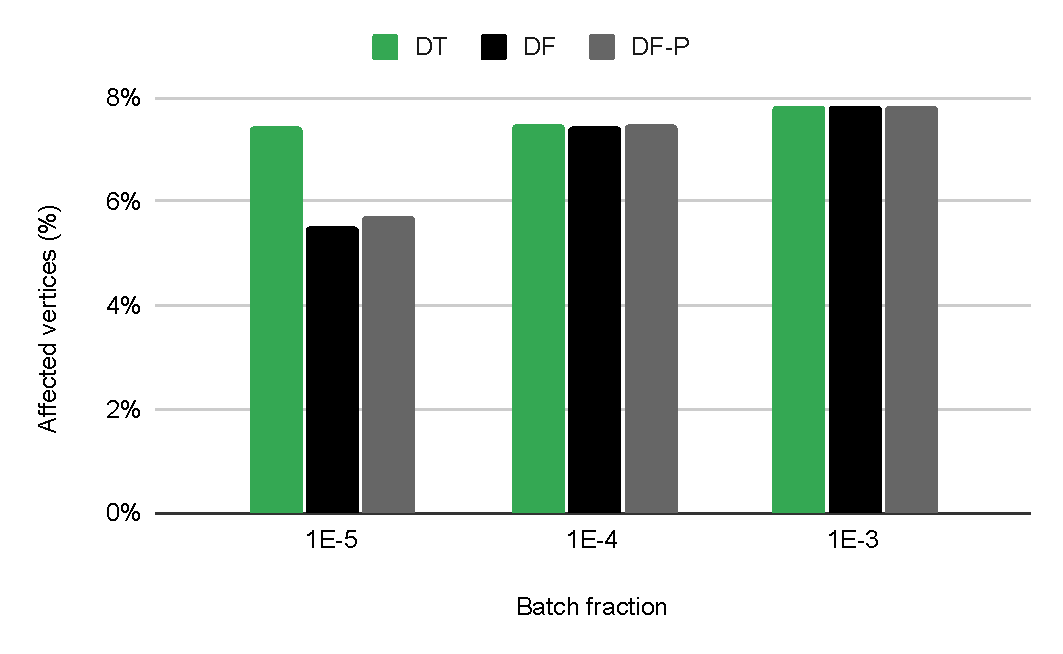
\includegraphics[width=0.98\linewidth]{out/measure-affected-batch.pdf}
  } \\[-2ex]
\caption{Average percentage of vertices marked as affected by \textit{Dynamic Traversal} and \textit{Dynamic Frontier} PageRank, with batch size increasing from $10^{-7} |E|$ to $0.1 |E|$ in multiples of $10$ (logarithmic scale), consisting purely of edge insertions. The \textit{Dynamic Frontier} approach marks affected vertices incrementally --- thus, the final percentage (at the end of all iterations) is depicted here.}
  \label{fig:measure-affected}
\end{figure}





\subsection{Performance of Dynamic Frontier PageRank}

We first study the performance of Dynamic Frontier PageRank on batch updates of size $10^{-7}|E|$ to $0.1|E|$ (in multiples of $10$), consisting purely of edge insertions, and compare it with Static, Naive-dynamic, and Dynamic Traversal PageRank. As mentioned above, the edge insertions are generated uniformly at random. Figure \ref{fig:insertions-runtime} plots the runtime of Static, Naive-dynamic, Dynamic Traversal, and Dynamic Frontier PageRank; Figure \ref{fig:insertions-speedup} plots the speedup of Dynamic Frontier PageRank with respect to Static, Naive-dynamic, and Dynamic Traversal PageRank; and Figure \ref{fig:insertions-error} plots the error in ranks obtained with Static, Naive-dynamic, Dynamic Traversal, and Dynamic Frontier PageRank with respect to ranks obtained from a reference Static PageRank (see Section \ref{sec:measurement}). In a similar manner, Figures \ref{fig:deletions-runtime}, \ref{fig:deletions-speedup}, and \ref{fig:deletions-error} present the runtime, speedup, and rank errors of each approach on batch updates consisting purely of edge deletions. Finally, Figures \ref{fig:8020-runtime}, \ref{fig:8020-speedup}, and \ref{fig:8020-error} present the runtime, speedup, and error with each approach on batch updates consisting of an $80\%$ / $20\%$ mix of edge insertions and deletions, in order to simulate realistic batch updates.


\subsubsection{Results with insertions-only batch updates}

Dynamic Frontier PageRank is on average $8.3\times$, $2.7\times$, and $3.4\times$ faster than Static, Naive-dynamic, and Dynamic Traversal PageRank on insertions-only batch updates of size $10^{-7}|E|$ to $10^{-3}|E|$, while obtaining ranks of better accuracy/error than Static PageRank, and of similar accuracy/error as Naive-dynamic and Dynamic Traversal PageRank. On road networks, and protein k-mer graphs, Dynamic Frontier PageRank is significantly faster than its competitors (Naive-dynamic and Dynamic Traversal PageRank).


\subsubsection{Results with deletions-only batch updates}

On deletions-only batch updates of size $10^{-7}|E|$ to $10^{-3}|E|$, Dynamic Frontier PageRank is on average $7.4\times$, $3.1\times$, and $4.1\times$ faster than Static, Naive-dynamic, and Dynamic Traversal PageRank, while obtaining ranks of better accuracy/error than Static PageRank (for batch sizes less than $0.1|E|$), and of similar accuracy/error as Naive-dynamic and Dynamic Traversal PageRank. On \textit{indochina-2004}, \textit{webbase-2001}, road networks, and protein k-mer graphs, Dynamic Frontier PageRank is significantly faster than its competitors (Naive-dynamic and Dynamic Traversal PageRank).


\subsubsection{Results with 80\%-20\% mix batch updates}

On batch updates of size $10^{-7}|E|$ to $10^{-3}|E|$, consisting of $80\%$ insertions and $20\%$ deletions, Dynamic Frontier PageRank is on average $7.6\times$, $2.8\times$, and $4.1\times$ faster than Static, Naive-dynamic, and Dynamic Traversal PageRank, while obtaining ranks of better accuracy/error than Static PageRank, and of similar accuracy/error as Naive-dynamic and Dynamic Traversal PageRank. Similar to deletions-only batch updates, Dynamic Frontier PageRank outperforms its competitors (Naive-dynamic and Dynamic Traversal PageRank) on \textit{indochina-2004}, \textit{webbase-2001}, road networks, and protein k-mer graphs.
% This seems to be associated to sparsity of the graphs as Dynamic Frontier PageRank performing well on sparse graphs.


\subsubsection{Results with temporal graphs}

We also attempt Static, Naive-dynamic, Dynamic Traversal, and Dynamic Frontier PageRank on temporal graphs found in the Stanford Large Network Dataset Collection \cite{snap14}. On some temporal graphs, Dynamic Frontier PageRank does not outperform its competitors with a frontier tolerance of $\tau_f = \tau / 10^5$, where $\tau$ is the iteration tolerance. However, choosing a lower $\tau_f$ of $\tau / 10$ or $\tau / 100$ allows it achieve good performance. Thus, the choice of frontier tolerance $\tau_f$, possibly in addition to how the frontier of affected vertices is expanded, is dependent upon the nature of the batch update. We plan to explore this in the future.


\subsubsection{Comparison of vertices marked as affected}

Figure \ref{fig:measure-affected} shows the total number of vertices marked as affected (average) by Dynamic Traversal and Dynamic Frontier PageRank on batch updates of size $10^{-7}|E|$ to $0.1|E|$, consisting exclusively of edge insertions. The Dynamic Frontier approach marks affected vertices incrementally --- thus, the final percentage (at the end of all iterations) is depicted in the figure. It is observed that Dynamic Traversal PageRank marks a higher percentage of vertices as affected, even for small batch updates.\ignore{This is likely due the randomly generated edges in the batch update being part of large Strongly Connected Components (SCCs), or due to a large number of such SCCs being reachable from the vertices that are part of the batch update.} In contrast, Dynamic Frontier PageRank marks far fewer vertices as affected, as it incrementally expands the affected region of the graph only after the rank of an affected vertex changes by a substantial amount, i.e., by frontier tolerance $\tau_f = \tau / 10^5$, where $\tau$ is the iteration tolerance (using $L\infty$-norm). In addition, as Dynamic Frontier PageRank incrementally marks vertices as affected, the actual work performed by the algorithm is lower than that indicated by the percentage of affected vertices in Figure \ref{fig:measure-affected}.

\begin{figure}[!hbt]
  \centering
  \subfigure{
    \label{fig:strong-scaling--speedup}
    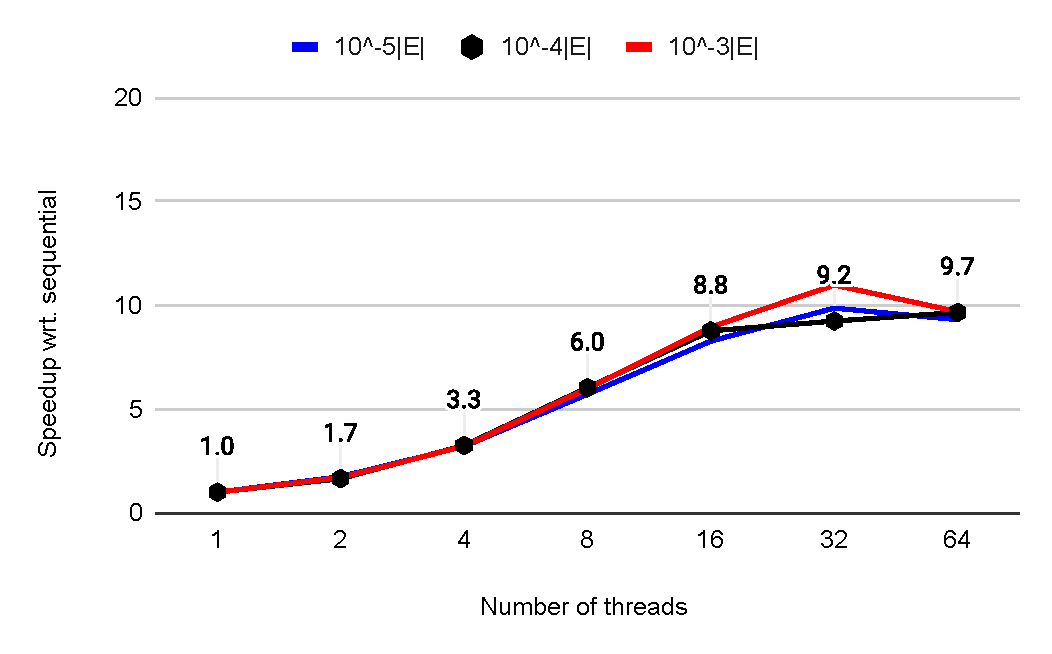
\includegraphics[width=0.98\linewidth]{out/strong-scaling-speedup.pdf}
  } \\[-2ex]
  \caption{Mean speedup of \textit{Dynamic Frontier (DF)} PageRank with increasing number of threads (in multiples of $2$), on real world dynamic graphs, with batch sizes of $10^{-5}|E|$ to $10^{-3}|E|$\ignore{ (consisting purely of edge insertions)}.}
  \label{fig:strong-scaling}
\end{figure}
%% TODO: Update this





\subsection{Strong Scaling of Dynamic Frontier PageRank}

Finally, we study the strong-scaling behavior of Dynamic Frontier PageRank on batch updates of a fixed size of $10^{-4} |E|$, consisting purely of edge insertions. Here, we measure the speedup of Dynamic Frontier PageRank with an increasing number of threads from $1$ to $64$ in multiples of $2$ with respect to a single-threaded execution of the algorithm. This is repeated for each graph in the dataset, and the results are averaged (using geometric mean).

The results are shown in Figure \ref{fig:strong-scaling}. With $16$ threads, Dynamic Frontier PageRank achieves an average speedup of $10.3\times$, compared to a single-threaded execution, indicating a performance increase of $1.8\times$ for every doubling of threads. At $32$ and $64$ threads, Dynamic Frontier PageRank is affected by NUMA effects (the $64$-core processor we use has $4$ NUMA domains), resulting in a speedup of only $14.3\times$ and $15.2\times$ respectively.

\ignore{\begin{figure}[!hbt]
  \centering
  \subfigure{
    \label{fig:weak-scaling--speedup}
    \includegraphics[width=0.98\linewidth]{out/weak-scaling-speedup.pdf}
  } \\[-2ex]
  \caption{Average speedup of \textit{Dynamic Frontier} PageRank with increasing number of threads (in multiples of $2$), on a batch sizes of $10^{-4}|E|$ to $6.4\times10^{-3}|E|$ (consisting purely of edge insertions), increasing in multiples of $2$ in tandem with the increase in the number of threads.}
  \label{fig:weak-scaling}
\end{figure}
}


\section{Conclusion}
\label{sec:conclusion}
In conclusion, this study presents an efficient algorithm for updating PageRank on dynamic graphs. Given a batch update of edge insertions and deletions, our Dynamic Frontier approach identifies an initial set of affected vertices and incrementally expands this set through iterations. On a server with a 64-core AMD EPYC-7742 processor, Dynamic Frontier PageRank outperforms Static, Naive-dynamic, and Dynamic Traversal PageRank by $8.3\times$, $2.7\times$, and $3.4\times$ respectively for uniformly random batch updates of size $10^{-7}|E|$ to $10^{-3}|E|$ with purely edge insertions; $7.4\times$, $3.1\times$, and $4.1\times$ respectively for purely edge deletion updates; and $7.6\times$, $2.8\times$, and $4.1\times$ for updates consisting of an $80\%$ - $20\%$ mix of insertions and deletions. Additionally, the approach exhibits a performance improvement of $1.8\times$ for each doubling of threads. On temporal graphs, we observe that lowering $\tau_f$ to $\tau / 10$ or $\tau / 100$ is needed for Dynamic Frontier PageRank to achieve food performance. Thus, a suitable choice of $\tau_f$ and how the frontier of affected vertices expands depend on the batch update's nature. We plan to explore this in the future.


%% The acknowledgments section.
\begin{acks}
I would like to thank Prof. Kishore Kothapalli, Prof. Sathya Peri, and Prof. Hemalatha Eedi for their support.
\end{acks}

%% Bibliography style to be used, and the bibliography file.
\bibliographystyle{ACM-Reference-Format}
\bibliography{main}

\end{document}
\endinput
%% End of file.




%% NOTES:
%% - Parallelization seems to be not efficient for small batch updates.
%% - Discuss about conflicting updates
%% - 


%% TODO:
%% - Scale up the size of the graphs
%% - Move experiments to a better server
%% - Include a weak- and strong- scalabiilty plot: run the expt from 2 to 128 threads
%% - overall space planning
%% - add a few lines on novelty of the paper.
%% - table comparison of related work
%% - Include a section on preliminaries that talks about the various algorithmic ideas (Louvain, Label Propagation)

%% Workplan:
%% - KK -- Read Introduction, Related Work,
%% - Dip Sankar -- Approach -- summarize the main algorithmic ideas,
%% - Subhajit -- Results -- Plots, scalability, Dataset, experiments, implementation details,
